\chapter{Distribuciones de probabilidad}

\textbf{Propósito:} Entender los concepto de variable aleatoria, función de densidad.


%%%%%%%%%%%%%%%%%%%%%%%%%%%%%%%%%%%%%%%%%%%%%%%
\subsection{Variable aleatoria}

\begin{definition}
Dado $A\subseteq \Omega$, la función indicadora de $A$ es la función con dominio $\Omega $ y contradominio $\{0,1\}$, es decir, 
\begin{equation*}
I_{A}(\omega )=\left\{ 
\begin{array}{c}
1\text{, si }\omega \in A \\ 
0\text{, si }\omega \notin A
\end{array}
\right.
\end{equation*}
\end{definition}

\begin{definition}[Variable aleatoria]
Para un espacio de probabilidad dado ($\Omega,S,P(\cdot ))$ una variable aleatoria $X$ o $X(\cdot)$ es una función con dominio $\Omega $ y contradominio la recta real, 
\begin{equation*}
X:\Omega \rightarrow  \mathbb{R}
\end{equation*}
\end{definition}

La función $X(\cdot)$ debe cumplir que para cada conjunto $A_{x}$ de la forma 
\begin{equation*}
A_{x}=\{\omega \in \Omega :X(\omega )\leq x\}
\end{equation*}
$A_{x}\in S$, esto  $\forall x\in \mathbb{R}$.

Observaciones:
\begin{enumerate}
\item Si $\Omega $ es finito o numerable, entonces $X(\omega ):\Omega \rightarrow \mathbb{Z}$, en este caso $\Omega $ es discreto. Note que el rango de $X$\ también sería finito o numerable.

\item Si $\Omega $ es no numerable, entonces $X(\omega ):\Omega \rightarrow \mathbb{R}$, en este caso $\Omega $ es continuo. Note que el rango de $X$ también sería  no numerable.
\end{enumerate}

\begin{example}
Experimento: Se lanza una moneda una vez. 
\vspace{5mm}

Los posibles resultados del experimento son: $a$, $s$. Sea $X$ la v.a que denota el número de veces que cae águila.

Entonces el espacio muestral está dado por
\begin{equation*}
\Omega =\{a,s\}
\end{equation*}
Como $X$ denota el número de veces que cae águila, se tiene que:
\begin{center}
\begin{tabular}{cc}
\hline
$\omega \in \Omega $ & $X(\omega )$ \\ 
\hline
s & $0$ \\ 
a & $1$ \\
\hline
\end{tabular}
\end{center}
Luego el \textit{soporte} (rango) de la variable aleatoria $X$ está dado por $\mathcal{X}=\{0,1\}\subset \mathbb{R}$.
\end{example}

\begin{remark}
Este ejemplo denota una variable aleatoria Bernoulli.
\end{remark}


\begin{example}
Experimento: Se lanza una moneda tres veces. Sea $X$ la v.a que denota el número de veces que cae águila en los tres lanzamientos.
Los resultado del experimento son: $sss$, $ssa$, $sas$, $ass$, $saa$, $asa$, $aas$, $aaa$. Entonces el espacio muestral del experimento está dado por
\begin{equation*}
\Omega =\{sss,\text{ }ssa,\text{ }sas,\text{ }ass,\text{ }saa,\text{ }asa,%
\text{ }aas,\text{ }aaa\}
\end{equation*}

La v.a $X$ denota el número de veces que cae águila en los tres lanzamientos:
\begin{center}
\begin{tabular}{cc}
\hline
$\omega \in \Omega $ & $X(\omega )$ \\
\hline
sss & $0$ \\ 
ssa & $1$ \\ 
sas & $1$ \\ 
ass & $1$ \\ 
saa & $2$ \\ 
asa & $2$ \\ 
aas & $2$ \\ 
aaa & $3$ \\
\hline
\end{tabular}
\end{center}

Entonces $\mathcal{X}=\{0,1,2,3\}$, note que $X(\cdot)$ asocia a cada resultado del experimento un número, de tal forma que
\begin{equation*}
X(\omega ):\Omega \rightarrow \mathcal{X}\subset \mathbb{R}
\end{equation*}
\end{example}


\begin{example}
Experimento: Se lanza una moneda $n$ veces. Sea $X$ la v.a que denota el número de veces que cae águila en los $n$ lanzamientos (Binomial). 

Por la regla de la multiplicación, la cardinalidad de $\Omega $ es $2^{n}$.

La v.a $X$ denota el número de águilas que se tienen en los $n$ lanzamientos:
\begin{center}
\begin{tabular}{cc}
\hline
$\omega \in \Omega $ & $X(\omega )=x$ \\ \hline
ssss... & $0$ \\ 
sass... & $1$ \\ 
ssas... & $1$ \\ 
$\vdots $ & $\vdots $ \\ 
aass... & $2$ \\ 
$\vdots $ & $\vdots $ \\ 
aaas... & $3$ \\ 
$\vdots $ & $\vdots $ \\ 
a$\cdots $a & $n$ \\ \hline
\end{tabular}
\end{center}

El soporte de la variable aleatoria $X$ está dado por $\mathcal{X}=\{0,1,2,3,...,n\}$.
\end{example}

\begin{remark}
Este ejemplo denota una variable aleatoria Binomial.
\end{remark}


%\begin{example}
%Experimento: Lanzamiento de una moneda, resultados águila y sol. La v.a  $X$ representa el número fallas antes del r-ésimo éxito (Binomial Negativa).
%\end{example}


%%%%%%%%%%%%%%%%%%%%%%%%%%%%%%%%%%%%%%%%%%%%%%%%%
\subsubsection{Práctica con R}


Lanzamiento de una moneda:
\begin{lstlisting}[language=R]
       coin1 <- coin()
       coin1
       toss(coin1)
\end{lstlisting}

Lanzamiento de una moneda tres veces:
\begin{lstlisting}[language=R]
       toss(coin1, times = 3)
\end{lstlisting}

%%%%%%%%%%%%%%%%%%%%%%%%%%%%%%%%%%%%%%%%%%%%%%%%%
\subsection{Función de masa de probabilidad}

\begin{definition}[v.a discreta]
Una v.a $X$ es discreta si el rango de la v.a $X$ es contable.
\end{definition}


Observaciones:
\begin{enumerate}

\item Que el rango de la v.a $X$ sea contable, significa que $\mathcal{X}$ es finito o numerable.

\item Si $X$ es discreta, i.e $\mathcal{X}=\{x_{1},x_{2},...\}$ entonces 
\begin{equation*}
\Omega =\bigcup\limits_{i}\{\omega :X(\omega
)=x_{i}\}=\bigcup\limits_{i}\{X=x_{i}\}
\end{equation*}%
donde $\{X=x_{i}\}\cap \{X=x_{j}\}=\varnothing $ para todo $i\neq j.$ 
Luego 
\begin{equation*}
P(\Omega )=\sum\limits_{i}P(X=x_{i})=1\text{, \ //Axioma 3}
\end{equation*}
\end{enumerate}

\begin{definition}[pmf]
Si $X$ es una v.a discreta con valores distintos $x_{1},x_{2},...,x_{n},$ entonces
\begin{equation*}
f_{X}(x)=\left\{ 
\begin{array}{l}
P(X=x)\text{, si }x=x_{j}\text{, \ }j=1,2,...,n \\ 
0,\text{ si }x\neq x_{j}
\end{array}
\right.
\end{equation*}
$f_{X}(x)$ es la función de masa de probabilidad (\textbf{pmf}) de $X$.
\end{definition}
 
\begin{remark}
$f_{X}(x)$ es una función con dominio $\mathcal{X}$ $\ \subset \mathbb{R}$ y contradominio $[0,1].$    
\end{remark}

\begin{example}
Experimento: Se lanza una moneda tres veces. Sea $X$ la variable aleatoria que denota el número de veces que cae águila en los tres lanzamientos.

Resultado:
\begin{center}
\begin{tabular}{c|c|c}
\hline
$\omega \in \Omega $ & $X(\omega )$ & $P(X(\omega )=x)$ \\ \hline
sss & $0$ & $P(X(\omega )=0)=1/8$ \\ 
ssa & $1$ & $P(X(\omega )=1)=1/8$ \\ 
sas & $1$ & $P(X(\omega )=1)=1/8$ \\ 
ass & $1$ & $P(X(\omega )=1)=1/8$ \\ 
saa & $2$ & $P(X(\omega )=2)=1/8$ \\ 
asa & $2$ & $P(X(\omega )=2)=1/8$ \\ 
aas & $2$ & $P(X(\omega )=2)=1/8$ \\ 
aaa & $3$ & $P(X(\omega )=3)=1/8$ \\ \hline
\end{tabular}
\end{center}

La pmf está dada por

\begin{center}
\begin{tabular}{c|c}
\hline
$x\in \chi $ & $f_{X}(x)=P(X=x)$ \\ \hline
$0$ & $P(X=0)=1/8$ \\ 
$1$ & $P(X=1)=3/8$ \\ 
$2$ & $P(X=2)=3/8$ \\ 
$3$ & $P(X=3)=1/8$ \\ \hline
\end{tabular}
\end{center}
\end{example}

\begin{figure}[h!]
\centering
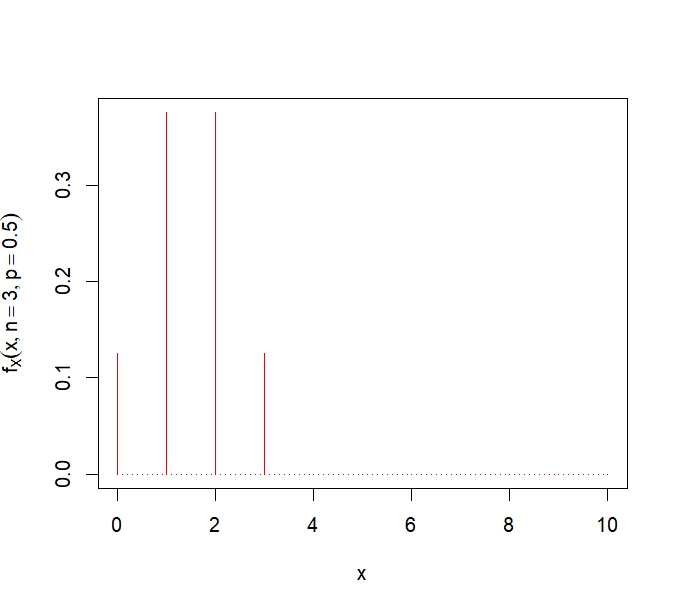
\includegraphics[scale=1]{Figuras/Binomial_n3.jpeg}
\caption{Función de masa de probabilidad binomial}
\end{figure}


\begin{example}
Experimento: Se lanza una moneda una vez, los resultados son águila y sol. La v.a  $X$ representa el número de lanzamientos requeridos hasta obtener del primer éxito (Geométrica).
\vspace{5mm}

La serie de ensayos son independientes teniendo cada ensayo dos posibles resultados: éxito o fracaso. Sea $p=P($ el ensayo termina en éxito$)$.

\vspace{5mm}
De acuerdo con lo anterior se tiene lo siguiente
\begin{eqnarray*}
f_{X}(x) &=&P(X=k) \\
&=&P(\text{ el primer éxito ocurre en el k-ésimo ensayo}) \\
&=&P(\text{en los primeros (k-1) ensayos se tienen fracasos})P(\text{k-ésimo ensayo se tiene éxito}) \\
&=&P(\text{(}k-1\text{) fracasos})P(\text{el k-ésimo es éxito}) \\
&=&(1-p)^{k-1}p
\end{eqnarray*}
Luego $f_{X}(x)=(1-p)^{k-1}p$,  $k=1,2,...$
\end{example}

\begin{remark}
Este ejemplo denota una variable aleatoria Geométrica.
\end{remark}

\begin{definition}[Propiedades de la pmf]
Cualquier función con dominio $\mathbb{R}$ y contradominio $[0,1]$ es una función de densidad discreta si para algún conjunto contable, $x_{1},x_{2},...,x_{n},...$ se tiene que:
\begin{enumerate}
\item $f(x)=0,$ si $x\neq x_{j}$, $j=1,2,3....$
\item $f(x)>0$, si $x=x_{j}$, $j=1,2,3,...$
\item $\sum f(x_{j})=1$
\end{enumerate}
\end{definition}

\vspace{5mm}
\textbf{pmf Bernoulli}: Un experimento Bernoulli tiene exactamente dos posibles resultados, éxito o fracaso. Una v.a Bernoulli $X$ tiene la función de masa de probabilidad 
\begin{equation*}
P(X=1)=p\text{ y }P(X=0)=1-p
\end{equation*}%
donde $p$ es la probabilidad de éxito.

La función de masa de probabilidad para una v.a Bernoulli, también se puede escribir de la siguiente forma
\begin{equation*}
f_{X}(x;p)=P(X=x)=p^{x}(1-p)^{1-x}I_{\{0,1\}}(x)
\end{equation*}

es decir, 
\begin{equation*}
f(x;p)=p^{x}q^{1-x}\text{, \ }x=0,1
\end{equation*}%
donde $0\leq p\leq 1$ y $q=1-p.$

\vspace{5mm}
\textbf{pmf Binomial:} Si $X$ registra el número de éxitos de $n$ ensayos Bernoulli independientes e idénticamente distribuidos (iid), con probabilidad de éxito $p.$ Entonces $X$ tiene función de masa de probabilidad Binomial($n,p$) dada por 
\begin{equation*}
f_{X}(x;p,n)=P(X=x)=\left( 
\begin{array}{c}
n \\ 
x
\end{array}
\right) p^{x}(1-p)^{n-x}
\end{equation*}%
donde $x=0,1,...,n.$

En otras palabras: 
\begin{equation*}
f(x;p,n)=\left( 
\begin{array}{c}
n \\ 
x
\end{array}%
\right) p^{x}q^{n-x}\text{, \ }x=0,1,2,...,n
\end{equation*}%
donde $0\leq p\leq 1$ y $q=1-p$, donde $p+q=1.$

\vspace{5mm}
\textbf{pmf Multinomial}: en un experimento dado con $n$ ensayos; para cada ensayo ocurren $k$ eventos mutuamente disjuntos $A_{1},...,A_{k}$ con probabilidad $P(A_{j})=p_{j}$, \ $j=1,...,k$.

Note que, si en un pmf binomial se tienen $n$ ensayos Bernoulli con dos posibles resultados y la probabilidad de éxito, $p$, es la misma en cada ensayo, en la pmf multinomial se tienen $n$ ensayos y en cada ensayo se tienen $k$ posibles resultados con probabilidades $P(A_{j})=p_{j}$,  $j=1,...,k$.

Dada $X_{j}$ la v.a que registra el número de veces que el evento $A_{j}$ ocurre en los $n$ ensayos idénticos e independientes del experimento. Entonces la función de masa de probabilidad está dada por
\begin{eqnarray*}
f(x_{1},x_{2},...,x_{k};p_{1},...,p_{k},n) &=&\left( 
\begin{array}{c}
n \\ 
x_{1},\text{ }x_{2},...,\text{ }x_{k}
\end{array}%
\right) p_{1}^{x_{1}}p_{2}^{x_{2}}\cdots p_{k}^{x_{k}} \\
&=&\frac{n!}{x_{1}!x_{2}!\cdots x_{k}!}p_{1}^{x_{1}}p_{2}^{x_{2}}\cdots
p_{k}^{x_{k}}
\end{eqnarray*}%
donde $\sum_{j=1}^{k}p_{k}=1$ y $\sum_{j=1}^{k}x_{j}=n$ con $0\leq x_{j}\leq
n$.

\vspace{5mm}
\textbf{pmf Uniforme}: 
\begin{equation*}
f(x;N)=\frac{1}{N}\text{, \ }x=1,2,...N
\end{equation*}

$N=1,2,...$
\vspace{5mm}
\textbf{pmf Poisson}
\begin{equation*}
f(x;\lambda )=\frac{e^{-\lambda }\lambda ^{x}}{x!}\text{, \ \ }x=0,1,2,...,
\end{equation*}%
donde $0\leq \lambda <\infty$.

\vspace{5mm}
\textbf{pmf Geométrica}: 
\begin{equation*}
f_{X}(x;p)=pq^{x-1}\text{ \ \ }x=1,2,..
\end{equation*}%
donde $0\leq p\leq 1$ y $q=1-p$


%%%%%%%%%%%%%%%%%%%%%%%%%%%%%%%%%%%%%%%%%%%%%
\subsection{Función de densidad de probabilidad}

\begin{definition}[pdf]
Si $X$ es una variable aleatoria continua, a su función $f_{X}(\cdot)$  se le llama función de densidad de probabilidad (\textbf{pdf}), y cumple con
\begin{equation*}
F_{X}(x)=\int_{-\infty }^{x}f_{X}(u)du
\end{equation*}
\end{definition}

\begin{definition}[Propiedades de la pdf]
Cualquier función $f_{X}(\cdot )$ con dominio $\mathbb{R}$ y contradominio $[0,\infty )$ es una función de densidad de probabilidad si y solo sí:
\begin{enumerate}
\item $f_{X}(x)\geq 0,$ $\forall x$
\item $\int_{-\infty }^{\infty }f_{X}(x)dx=1$
\end{enumerate}
\end{definition}

\textbf{pdf t}: William Sealy Gosset era un matemático y químico inglés que después de terminar sus estudios comenzó a trabajar en las destilerías Guinness, en lo que se refiere a control de calidad en el proceso de creación de la cerveza. Los tamaños pequeños de las muestras con los que habitualmente contaba fueron los responsables de sus estudios, y los que a la postre lo llevaron a desarrollar la distribución t. En $1908$, publico el artículo $\emph{The}$ $\emph{probable}$ $\emph{error}$ $\emph{of}$ $\emph{a}$ $\emph{mean}$ en la revista Biometrika con el seudónimo Student. La distribución $t$ de Student es una distribución de probabilidad que aparece cuando se quiere estimar la media de una población cuando el tamaño de la muestra utilizada para la estimación es pequeña y la varianza de la población es desconocida.


La distribución de probabilidad $t$ está dada por
\begin{equation*}
f_{X}(x;k)=\frac{\Gamma ((k+1)/2)}{\Gamma (k/2)}\frac{1}{\sqrt{k\pi }}\frac{1
}{\left( 1+\frac{x^{2}}{k}\right) ^{(k+1)/2}}\text{, }-\infty <x<\infty
\end{equation*}
donde $k>0.$

\textbf{pdf uniforme}: 
\begin{equation*}
f(x;a,b)=\frac{1}{b-a}\text{, \ }x\in \lbrack a,b]
\end{equation*}%
donde $-\infty <a<b<\infty$.

\textbf{pdf exponencial}:
\begin{equation*}
f(x;\lambda )=\lambda e^{-\lambda x}\text{ }x\in (0,\infty )
\end{equation*}%
donde $\lambda >0.$


\textbf{pdf normal:}
\begin{equation*}
f_{X}(x;\mu ,\sigma )=\frac{1}{\sqrt{2\pi \sigma ^{2}}}e^{-\frac{1}{2}\left( 
\frac{x-\mu }{\sigma }\right) ^{2}}
\end{equation*}
donde $-\infty <\mu <\infty $, \ $\sigma >0$ y $-\infty <x<\infty $


\textbf{pdf Cauchy:}
\begin{equation*}
f_{X}(x;\mu ,\sigma )=\frac{1}{\pi \beta \left[ 1+\left( \frac{x-\alpha }{%
\beta }\right) ^{2}\right] }
\end{equation*}
donde $-\infty <\alpha <\infty $, \ $\beta >0$ y $-\infty <x<\infty $


%%%%%%%‰%%%%%%%%%%%%%%%%%%%%%%%%%%%%%%%%
\subsection{Función de distribución acumulativa}

\begin{definition}[cdf]
La función de distribución acumulada (\textbf{cdf}) de una v.a $X$, es una función con dominio la recta real y contradominio el intervalo $[0,1]$,
\begin{equation*}
F_{X}:\mathbb{R}
\rightarrow \lbrack 0,1]
\end{equation*}
que satisface que 
\begin{eqnarray*}
F_{X}(x) &=&P(X\leq x) \\
&=&P(\{\omega \in \Omega :X(\omega )\leq x\})
\end{eqnarray*}
para todo $x\in \mathbb{R}$
\end{definition}

\vspace{5mm}
Una v.a $X$ continua tiene cdf, $F_{X},$ continua. Una variable aleatoria $X$ discreta tiene cdf, $F_{X},$ discreta, y es una función escalonada, "step".

\vspace{5mm}
\textbf{cdf v.a Discreta}: Dada $X$ una v.a discreta con $\mathcal{X}=\{x_{1},x_{2},...\}$ , la cdf $F_{X}(\cdot )$ puede ser obtenida de la pdf $f_{X}(\cdot )$ y viceversa; ya que 
\begin{equation*}
F_{X}(x)=\sum_{\{j\text{ }:\text{ }x_{j}\leq x\}}f_{X}(x_{j})
\end{equation*}
y 
\begin{equation*}
f_{X}(x_{j})=F_{X}(x_{j})-\lim_{0<h\rightarrow 0}F_{X}(x_{j}-h)
\end{equation*}

\textbf{cdf v.a Continua}: Dada $X$ una v.a continua, la cdf $F_{X}(\cdot )$ puede ser obtenida de la pdf $f_{X}(\cdot )$ y viceversa; ya que si $X$ es una v.a continua y $f_{X}(x)$ está dada, entonces $F_{X}(x)$ es obtenida a partir de integrar $f_{X}(x)$, es decir,
\begin{equation*}
F_{X}(x)=P(X\leq x)=\int_{-\infty }^{x}f_{X}(u)du
\end{equation*}


\section{Distribuciones de probabilidad de variables aleatorias discretas}

%%%%%%%%%%%%%%%%%%%%%%%%%%%%%%%%%%%%%%%%%%%%%%%
\subsection{Uniforme discreta}

\begin{definition}
La distribución uniforme discreta está dada por 
\begin{equation*}
f_{X}(x)=f_{X}(x;N)=P(X=x)=\left\{ 
\begin{array}{l}
1/N\text{, si }x\in \mathcal{X} \\ 
0,\text{ si }x\notin \mathcal{X}
\end{array}
\right.
\end{equation*}
es decir 
\begin{equation*}
f_{X}(x;N)=\frac{1}{N}I_{\{1,2,...,N\}}(x)
\end{equation*}
\end{definition}


\begin{i}

\begin{theorem}
Si $X$ tiene distribución uniforma discreta, entonces
\begin{equation*}
E(X)=\frac{N+1}{2}
\end{equation*}
\begin{equation*}
Var(X)=\frac{N^{2}-1}{12}
\end{equation*}
y 
\begin{equation*}
m_{X}(t)=\sum\limits_{j=1}^{N}e^{tj}\frac{1}{N}\text{ //}j=x
\end{equation*}
\end{theorem}

Demostración: Dado que

\begin{equation*}
E(X)=\sum x_{j}f_{X}(x_{j})
\end{equation*}%
entonces%
\begin{eqnarray*}
E(X) &=&\sum_{j=1}^{N}j\frac{1}{N}\text{ \ \ //}x=j \\
&=&\frac{1}{N}\sum_{j=1}^{N}j\text{ \ \ //inducción} \\
&=&\frac{1}{N}\frac{N(N+1)}{2}=\frac{N+1}{2}
\end{eqnarray*}

Luego 
\begin{equation*}
E(X)=\frac{N+1}{2}
\end{equation*}

Por otra parte, note que 
\begin{eqnarray*}
E(X^{2}) &=&\sum_{j=1}^{N}j^{2}\frac{1}{N}\text{ \ //}x=j \\
&=&\frac{1}{N}\sum_{j=1}^{N}j^{2}\text{ // inducción} \\
&=&\frac{1}{N}\frac{N(N+1)(2N+1)}{6} \\
&=&\frac{(N+1)(2N+1)}{6}
\end{eqnarray*}
Como 
\begin{equation*}
V(X)=E(X^{2})-[E(X)]^{2}
\end{equation*}
entonces
\begin{eqnarray*}
V(X) &=&\frac{(N+1)(2N+1)}{6}-\frac{\left( N+1\right) ^{2}}{4} \\
&=&(N+1)\left( \frac{2N+1}{6}-\frac{\left( N+1\right) }{4}\right) \\
&=&(N+1)\left( \frac{4N+2-3N-3}{12}\right) \\
&=&(N+1)\left( \frac{N-1}{12}\right) \\
&=&\frac{N^{2}-1}{12}
\end{eqnarray*}
luego
\begin{equation*}
V(X)=\frac{N^{2}-1}{12}
\end{equation*}

Finalmente
\begin{eqnarray*}
m_{X}(t) &=&E(e^{tX}) \\
&=&\sum\limits_{j=1}^{N}e^{tj}\frac{1}{N}\text{ //}x=j \\
&=&\frac{1}{N}\sum\limits_{j=1}^{N}e^{tj}
\end{eqnarray*}

%%%%%%%%%%%%%%%%%%%%%%%%%%%%%%%%%%%%%
\subsection{Bernoulli}

\begin{definition}
Una v.a $X$ tiene distribución Bernoulli si la pmf de $X$ está dada por 
\begin{equation*}
f_{X}(x)=f_{X}(x;p)=P(X=x)=\left\{ 
\begin{array}{l}
p^{x}(1-p)^{1-x}\text{, si }x\in \mathcal{X}=\{0,1\} \\ 
0\text{ si }x\notin \mathcal{X}
\end{array}
\right.
\end{equation*}
es decir
\begin{equation*}
f_{X}(x,p)=p^{x}(1-p)^{1-x}I_{\{0,1\}}(x)
\end{equation*}%
donde $0\leq p\leq 1.$ Si $q=1-p$, entonces
\begin{equation*}
f_{X}(x)=p^{x}q^{1-x}I_{\{0,1\}}(x)
\end{equation*}
\end{definition}

\begin{figure}[h!]
\centering
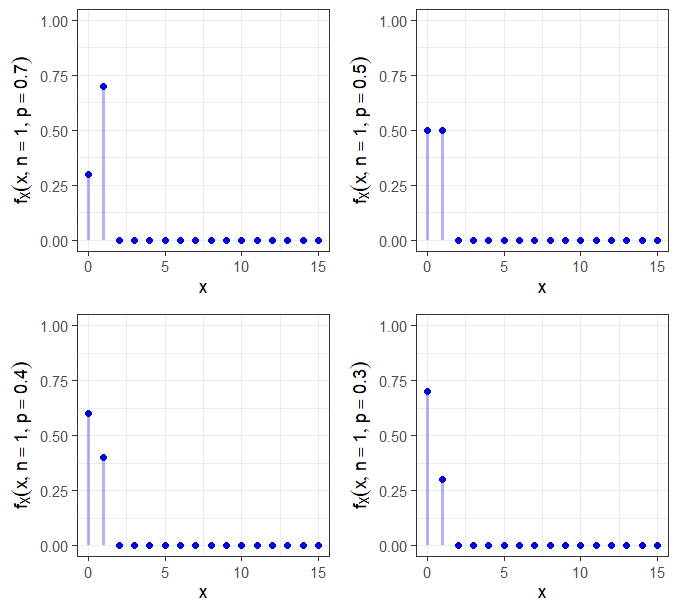
\includegraphics[scale=1]{Figuras/Bernoulli.jpeg}
\caption{Función de masa de probabilidad Bernoulli}
\end{figure}

\begin{theorem}
Si $X$ tiene distribución Bernoulli, entonces 
\begin{eqnarray*}
E(X) &=&p \\
V(X) &=&pq \\
m_{X}(t) &=&pe^{t}+q
\end{eqnarray*}
\end{theorem}

Demostración:
\begin{eqnarray*}
E(X) &=&\sum_{x\in \mathcal{X}}xf_{X}(x) \\
&=&\sum_{x\in \mathcal{X}}xp^{x}(1-p)^{1-x} \\
&=&0p^{0}(1-p)^{1-0}+1p^{1}(1-p)^{1-1} \\
&=&p
\end{eqnarray*}
Por lo tanto
\begin{equation*}
E(X)=p
\end{equation*}

Por otra parte 
\begin{eqnarray*}
E(X^{2}) &=&\sum_{x}x^{2}f_{X}(x) \\
&=&\sum_{x\in \mathcal{X}}x^{2}p^{x}(1-p)^{1-x} \\
&=&0^{2}p^{0}(1-p)^{1-0}+1^{2}p^{1}(1-p)^{1-1} \\
&=&p
\end{eqnarray*}
Entonces
\begin{eqnarray*}
V(X) &=&E(X^{2})-[E(X)]^{2} \\
&=&p-p^{2} \\
&=&p(1-p)\text{ //}q=1-p \\
&=&pq
\end{eqnarray*}
Por lo tanto
\begin{equation*}
V(X)=pq
\end{equation*}

Finalmente note que 
\begin{eqnarray*}
m_{X}(t) &=&E(e^{tX}) \\
&=&\sum_{x\in \mathcal{X}}e^{tx}f(x) \\
&=&\sum_{x=0}^{1}e^{tx}p^{x}(1-p)^{1-x} \\
&=&e^{t0}p^{0}(1-p)^{1-0}+e^{t}p^{1}(1-p)^{1-1} \\
&=&(1-p)+e^{t}p
\end{eqnarray*}
Por lo tanto
\begin{equation*}
m_{X}(t)=e^{t}p+q
\end{equation*}

%%%%%%%%%%%%%%%%%%%%%%%%%%%%%%%%%%%%%%
\subsection{Binomial}

\begin{definition}
Una v.a $X$ tiene distribución Binomial si la pmf de $X$ está dada por 
\begin{equation*}
f_{X}(x)=f_{X}(x;n,p)=P(X=x)=\left\{ 
\begin{array}{l}
\binom{n}{x}p^{x}q^{1-x}\text{, si }x\in \mathcal{X}=\{0,1,...,n\} \\ 
0,\text{ si }x\notin \mathcal{X}%
\end{array}%
\right.
\end{equation*}%
Es decir;
\begin{equation*}
f_{X}(x;n,p)=\binom{n}{x}p^{x}q^{1-x}I_{\{0,1,...,n\}}(x)
\end{equation*}%
donde $0\leq p\leq 1$, $q=1-p$.
\end{definition}

\begin{figure}[h!]
\centering
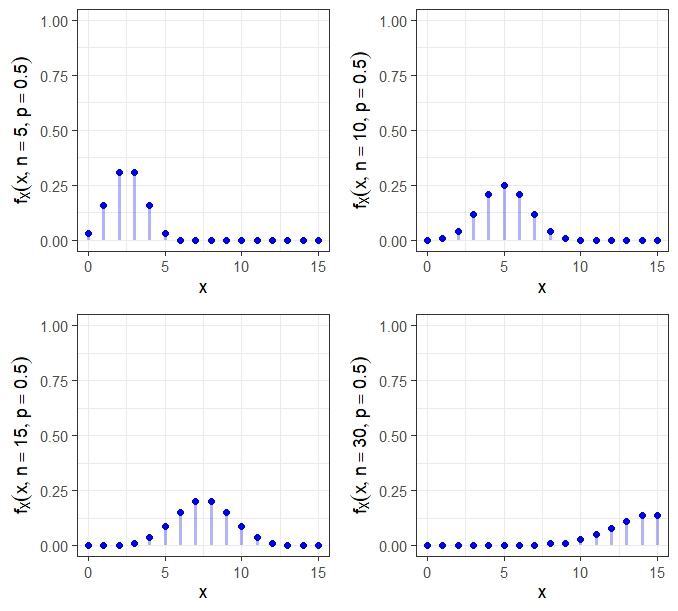
\includegraphics[scale=1]{Figuras/Binomial.jpeg}
\caption{Función de masa de probabilidad Binomial}
\end{figure}

\begin{theorem}
Si $X$ tiene distribución binomial, entonces
\begin{eqnarray*}
E(X) &=&np \\
V(X) &=&npq \\
m_{X}(t) &=&\left( q+pe^{t}\right) ^{n}
\end{eqnarray*}
\end{theorem}

Demostración: Se deduce primero la fgm 
\begin{eqnarray*}
m_{X}(t) &=&E(e^{tX}) \\
&=&\sum_{x}e^{tx}\binom{n}{x}p^{x}q^{1-x} \\
&=&\sum_{x=0}^{n}\binom{n}{x}\left( pe^{t}\right) ^{x}q^{1-x}\text{ //}
\sum_{j=0}^{n}\binom{n}{j}a^{j}b^{n-j}=(a+b)^{n} \\
&=&(pe^{t}+q)^{n}
\end{eqnarray*}
es decir, 
\begin{equation*}
m_{X}(t)=(pe^{t}+q)^{n}
\end{equation*}

Dado que 
\begin{equation*}
E(X)=\frac{d}{dt}m_{X}(t)
\end{equation*}

Entonces
\begin{equation*}
\frac{d}{dt}m_{X}(t)=n(pe^{t}+q)^{n-1}pe^{t}
\end{equation*}%
luego%
\begin{eqnarray*}
\left. \frac{d}{dt}m_{X}(t)\right\vert _{t=0} &=&n(pe^{0}+q)^{n-1}pe^{0} \\
&=&np
\end{eqnarray*}%
entonces
\begin{equation*}
E(X)=np
\end{equation*}

Por otra parte
\begin{equation*}
E(X^{2})=\frac{d^{2}}{dt^{2}}m_{X}(t)
\end{equation*}
Entonces
\begin{equation*}
\frac{d^{2}}{dt^{2}}
m_{X}(t)=n(n-1)(pe^{t}+q)^{n-2}p^{2}e^{2t}+pe^{t}n(pe^{t}+q)^{n-1}
\end{equation*}
luego
\begin{eqnarray*}
\left. \frac{d^{2}}{dt^{2}}m_{X}(t)\right\vert _{t=0}
&=&n(n-1)(pe^{0}+q)^{n-2}p^{2}e^{2(0)}+pe^{0}n(pe^{0}+q)^{n-1} \\
&=&n(n-1)(p+1-p)^{n-2}p^{2}+pn(p+1-p)^{n-1} \\
&=&n(n-1)p^{2}+pn
\end{eqnarray*}
entonces
\begin{equation*}
E(X^{2})=n(n-1)p^{2}+pn
\end{equation*}
Finalmente 
\begin{eqnarray*}
V(X) &=&E(X^{2})-[E(X)]^{2} \\
&=&n^{2}p^{2}-np^{2}+pn-n^{2}p^{2} \\
&=&pn-np^{2} \\
&=&n(p-p^{2}) \\
&=&n(p(1-p)) \\
&=&npq
\end{eqnarray*}
luego%
\begin{equation*}
V(X)=npq
\end{equation*}
%%%%%%%%%%%%%%%%%%%%%%%%%%%%%%%%%%%%%%%%%
\subsubsection{Resolución de problemas}

Para $X$, una variable aleatoria Binomial con $n=5$ y $p=0.5$, calcular su media y varianza.

\begin{figure}[h!]
\centering
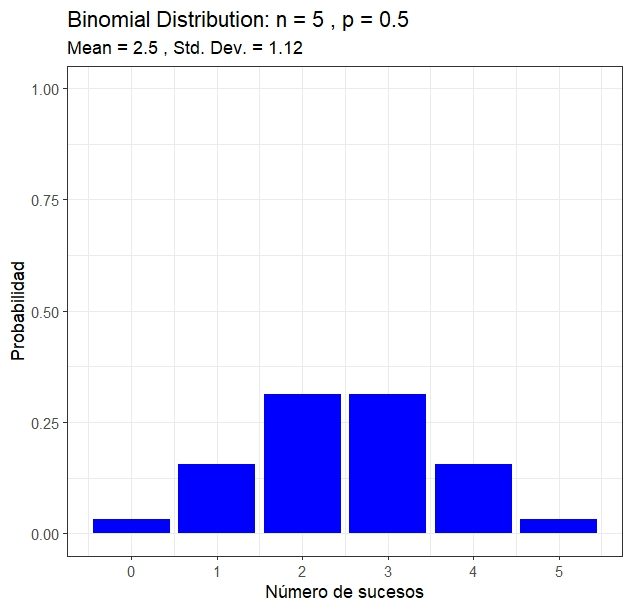
\includegraphics[scale=0.8]{Figuras/Binomial_n5.jpeg}
\caption{Función de masa de probabilidad Binomial}
\end{figure}

Para $X$, una variable aleatoria Binomial con $n=10$ y $p=0.5$, calcular su media y varianza. 

\begin{figure}[h!]
\centering
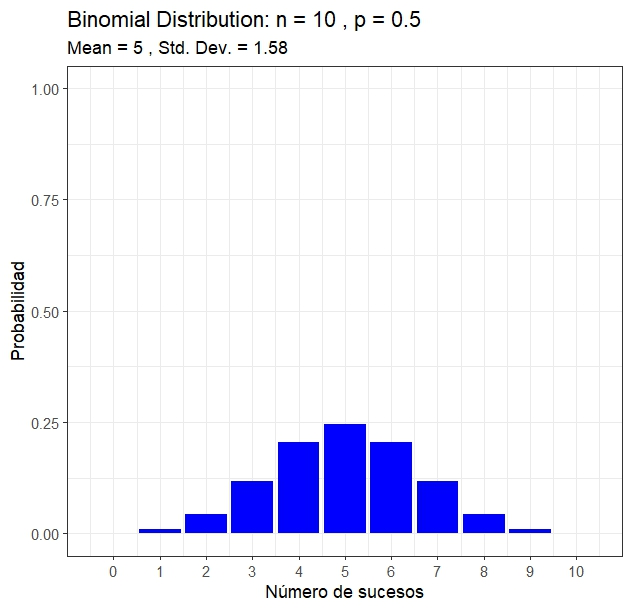
\includegraphics[scale=0.8]{Figuras/Binomial_n10.jpeg}
\caption{Función de masa de probabilidad Binomial}
\end{figure}


%%%%%%%%%%%%%%%%%%%%%%%%%%%%%%%%%%%%%%%%%
\subsubsection{Práctica con R}
%%%%%%%%%%%%%%%%%%%%%%%%%%%%%%%%%%%%%%%%%
% Agragar gráficos dinámicos


%%%%%%%%%%%%%%%%%%%%%%%%%%%%%%%%%%%%%%%%%%%%%%%%%%
\subsection{Hipergeométrica}

\begin{definition}
Una v.a $X$ tiene distribución hipergeométrica si su pmf está dada por 
\begin{equation*}
f_{X}(x,M,n,K)=\frac{\binom{K}{x}\binom{M-K}{n-x}}{\binom{M}{n}}\text{, }%
x=0,1,..,n
\end{equation*}
donde
$M=1,2,...$
$K=0,1,...,M$
$n=1,2,...,M$
\end{definition}

Note que 
\begin{equation*}
f_{X}(x,M,n,K)=\frac{\binom{K}{x}\binom{M-K}{n-x}}{\binom{M}{n}}
I_{\{0,1,...,n\}}(x).
\end{equation*}

\begin{figure}[h!]
\centering
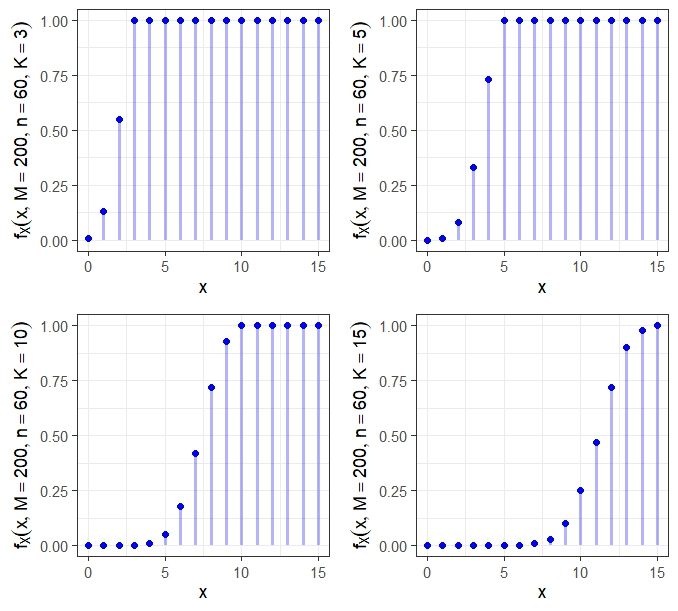
\includegraphics[scale=1]{Figuras/Hipergeometrica.jpeg}
\caption{Función de masa de probabilidad Hipergeométrica}
\end{figure}

\begin{theorem}
Si $X$ tiene distribución hipergeométrica, entonces
\begin{eqnarray*}
E(X) &=&n\frac{K}{M} \\
V(X) &=&n\cdot \frac{K}{M}\cdot \frac{M-K}{M}\cdot \frac{M-n}{M-1}
\end{eqnarray*}
\end{theorem}

Demostración
\begin{eqnarray*}
E(X) &=&\sum_{x}xf_{X}(x) \\
&=&\sum_{x=0}^{n}x\frac{\binom{K}{x}\binom{M-K}{n-x}}{\binom{M}{n}} \\
&=&\sum_{x=1}^{n}x\frac{\binom{K}{x}\binom{M-K}{n-x}}{\binom{M}{n}}
\end{eqnarray*}

Usando la función indicadora, note que 
\begin{equation*}
x\binom{K}{x}=x\frac{K!}{x!(K-x)!}=\frac{K!}{\left( x-1\right) !(K-x)!}=%
\frac{K(K-1)!}{\left( x-1\right) !(K-x)!}=K\binom{K-1}{x-1}
\end{equation*}

\begin{equation*}
\binom{M}{n}=\frac{M!}{n!(M-n)!}=\frac{M(M-1)!}{n(n-1)!(M-n)!}=\frac{M}{n}
\binom{M-1}{n-1}
\end{equation*}
Entonces
\begin{eqnarray*}
\sum_{x=1}^{n}x\frac{\binom{K}{x}\binom{M-K}{n-x}}{\binom{M}{n}}
&=&\sum_{x=1}^{n}\frac{K\binom{K-1}{x-1}\binom{M-K}{n-x}}{\frac{M}{n}\binom{
M-1}{n-1}} \\
&=&n\frac{K}{M}\sum_{x=1}^{n}\frac{\binom{K-1}{x-1}\binom{M-K}{n-x}}{\binom{
M-1}{n-1}}
\end{eqnarray*}

Sea $y=x-1$ entonces $x=y+1$, luego 
\begin{eqnarray*}
E(X) &=&n\frac{K}{M}\sum_{y=0}^{n-1}\frac{\binom{K-1}{y}\binom{M-1-K+1}{n-1-y%
}}{\binom{M-1}{n-1}}//pmf \\
&=&n\frac{K}{M}
\end{eqnarray*}

Por otra parte, el segundo momento factorial de $X$ está dado por%
\begin{eqnarray*}
E[X(X-1)] &=&\sum_{x=0}^{n}x(x-1)\frac{\binom{K}{x}\binom{M-K}{n-x}}{\binom{M%
}{n}} \\
&=&\sum_{x=2}^{n}x(x-1)\frac{\binom{K}{x}\binom{M-K}{n-x}}{\binom{M}{n}}
\end{eqnarray*}

Note que
\begin{eqnarray*}
x(x-1)\binom{K}{x} &=&x(x-1)\frac{K!}{x!(K-x)!} \\
&=&\frac{K(K-1)(K-2)!}{(x-2)!(K-x)!} \\
&=&K(K-1)\binom{K-2}{x-2}
\end{eqnarray*}
y 
\begin{equation*}
\binom{M}{n}=\frac{M!}{n!(M-n)!}=\frac{M(M-1)(M-2)!}{n(n-1)(n-2)!(M-n)!}=
\frac{M}{n}\cdot \frac{\left( M-1\right) }{\left( n-1\right) }\binom{M-2}{n-2
}
\end{equation*}
Sustituyendo
\begin{eqnarray*}
E[X(X-1)] &=&\sum_{x=2}^{n}\frac{K(K-1)\binom{K-2}{x-2}\binom{M-K}{n-x}}{%
\frac{M}{n}\frac{\left( M-1\right) }{\left( n-1\right) }\binom{M-2}{n-2}} \\
&=&n(n-1)\frac{K(K-1)}{M\left( M-1\right) }\sum_{x=2}^{n}\frac{\binom{K-2}{
x-2}\binom{M-K}{n-x}}{\binom{M-2}{n-2}}
\end{eqnarray*}

Sea $y=x-2$, entonces $x=y+2$, luego
\begin{equation*}
\sum_{y=0}^{n-2}\frac{\binom{K-2}{y}\binom{M-2-K+2}{n-2-y}}{\binom{M-2}{n-2}}
=1\text{ //pmf}
\end{equation*}
entonces
\begin{equation*}
E[X(X-1)]=n(n-1)\frac{K(K-1)}{M\left( M-1\right) }
\end{equation*}

Como
\begin{eqnarray*}
E[X(X-1)] &=&E[X^{2}-X] \\
&=&E(X^{2})-E(X)
\end{eqnarray*}
Entonces, despejando
\begin{equation*}
E(X^{2})=E[X(X-1)]+E(X)
\end{equation*}

Luego

\begin{eqnarray*}
V(X) &=&E(X^{2})-[E(X)]^{2}\text{ \ //Def.} \\
&=&E[X(X-1)]+E(X)-[E(X)]^{2} \\
&=&n(n-1)\frac{K(K-1)}{M\left( M-1\right) }+\frac{nK}{M}-\frac{n^{2}K^{2}}{
M^{2}} \\
&=&n\frac{K}{M}\left[ (n-1)\frac{(K-1)}{\left( M-1\right) }+1-\frac{nK}{M}
\right] \\
&=&n\frac{K}{M}\left[ (n-1)\frac{(K-1)}{\left( M-1\right) }+\frac{M-nK}{M}
\right] \\
&=&n\frac{K}{M}\left[ \frac{(n-1)(KM-M)+M^{2}-M-nKM+nK}{M\left( M-1\right) }%
\right] \\
&=&n\frac{K}{M}\frac{1}{M(M-1)}\left[ nKM-KM-nM+M+M^{2}-M-nKM+nK\right] \\
&=&n\frac{K}{M}\frac{1}{M(M-1)}\left( M^{2}-KM-nM+nK\right) \\
&=&n\frac{K}{M}\frac{1}{M(M-1)}(M-K)(M-n)
\end{eqnarray*}%
luego%
\begin{equation*}
V(X)=n\frac{K}{M}\cdot \frac{M-K}{M}\cdot \frac{M-n}{M-1}
\end{equation*}


%%%%%%%%%%%%%%%%%%%%%%%%%%%%%%%%%%%%%%%
\subsection{Poisson}

\begin{definition}
Una v.a $X$ tiene distribución Poisson, si 
\begin{equation*}
f(x;\lambda )=\frac{e^{-\lambda }\lambda ^{x}}{x!}I_{\{0,1,...\}}(x)
\end{equation*}%
con $\lambda >0.$
\end{definition}

\begin{figure}[h!]
\centering
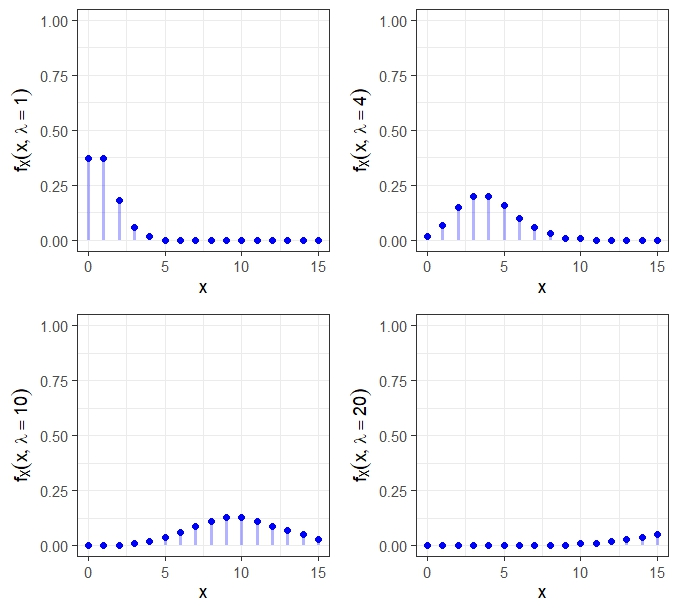
\includegraphics[scale=1]{Figuras/Poisson.jpeg}
\caption{Función de masa de probabilidad Poisson.}
\end{figure}

\begin{theorem}
Si la v.a $X$ tiene distribución Poisson, entonces
\begin{eqnarray*}
E(X) &=&\lambda \\
V(X) &=&\lambda \\
m_{X}(t) &=&e^{\lambda (e^{t}-1)}
\end{eqnarray*}
\end{theorem}

Demostración:
\begin{eqnarray*}
E(X) &=&\sum_{x}xf(x) \\
&=&\sum_{x=0}^{\infty }x\frac{e^{-\lambda }\lambda ^{x}}{x!} \\
&=&e^{-\lambda }\sum_{x=0}^{\infty }x\frac{\lambda ^{x}}{x!} \\
&=&\lambda e^{-\lambda }\sum_{x=1}^{\infty }\frac{\lambda ^{x-1}}{(x-1)!}
\end{eqnarray*}
sea $y=x-1$, entonces
\begin{eqnarray*}
E(X) &=&\lambda e^{-\lambda }\sum_{y=0}^{\infty }\frac{\lambda ^{y}}{y!}%
\text{ \ \ //}\sum_{j=0}^{\infty }\frac{x^{j}}{j!}=e^{x} \\
&=&\lambda e^{-\lambda }e^{\lambda } \\
&=&\lambda
\end{eqnarray*}
Por otra parte
\begin{eqnarray*}
E(X(X-1)) &=&\sum_{x=0}^{\infty }x(x-1)\frac{e^{-\lambda }\lambda ^{x}}{x!}
\\
&=&e^{-\lambda }\sum_{x=2}^{\infty }\frac{\lambda ^{x}}{(x-2)!} \\
&=&\lambda ^{2}e^{-\lambda }\sum_{x=2}^{\infty }\frac{\lambda ^{x-2}}{(x-2)!}
\end{eqnarray*}
sea $y=x-2$

entonces
\begin{eqnarray*}
E(X(X-1)) &=&\lambda ^{2}e^{-\lambda }\sum_{y=0}^{\infty }\frac{\lambda ^{y}%
}{y!} \\
&=&\lambda ^{2}e^{-\lambda }e^{\lambda } \\
&=&\lambda ^{2}
\end{eqnarray*}
Como 
\begin{eqnarray*}
V(X) &=&E(X(X-1))+E(X)-[E(X)]^{2} \\
&=&\lambda ^{2}+\lambda -\lambda ^{2} \\
&=&\lambda
\end{eqnarray*}
Luego 
\begin{equation*}
V(X)=\lambda
\end{equation*}

Por otra parte; 
\begin{eqnarray*}
m_{X}(t) &=&E(e^{tX}) \\
&=&\sum_{x=0}^{\infty }e^{tx}\frac{e^{-\lambda }\lambda ^{x}}{x!} \\
&=&e^{-\lambda }\sum_{x=0}^{\infty }\frac{\left( e^{t}\lambda \right) ^{x}}{
x!} \\
&=&e^{-\lambda }e^{\lambda e^{t}} \\
&=&e^{\lambda e^{t}}e^{-\lambda } \\
&=&e^{\lambda \left( e^{t}-1\right) }
\end{eqnarray*}

Por lo tanto
\begin{equation*}
m_{X}(t)=e^{\lambda \left( e^{t}-1\right) }
\end{equation*}


%%%%%%%%%%%%%%%%%%%%%%%%%%%%%%%%%%%%%%%%%%%
\subsection{Binomial negativa}

\begin{definition}
Una v.a $X$ con distribución binomial negativa, está dada por 
\begin{equation*}
f(x;r,p)=\binom{r+x-1}{x}p^{r}q^{x}=\binom{-r}{x}p^{r}(-q)^{x}\text{, \ \ \
\ }x=0,1,2,...
\end{equation*}
donde $0<p\leq 1,$ $q=1-p$ $\ $y $r=1,2,3,...$ 
\end{definition}

\begin{figure}[h!]
\centering
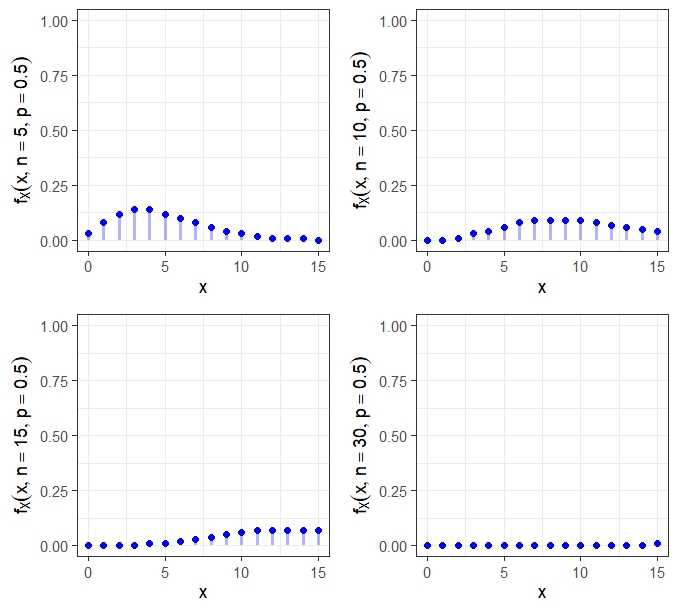
\includegraphics[scale=1]{Figuras/Binomial_negativa.jpeg}
\caption{Función de masa de probabilidad Binomial negatica}
\end{figure}


\begin{theorem}
Si $X$ tiene distribución binomial negativa, entonces
\begin{eqnarray*}
E(X) &=&\frac{rq}{p} \\
V(X) &=&\frac{rq}{p^{2}} \\
m_{X}(t) &=&\left( \frac{p}{1-qe^{t}}\right) ^{r}
\end{eqnarray*}
\end{theorem}

Demostración: 
\begin{eqnarray*}
m_{X}(t) &=&E(e^{tX}) \\
&=&\sum_{x=0}^{\infty }e^{tx}\binom{-r}{x}p^{r}(-q)^{x} \\
&=&\sum_{x=0}^{\infty }\binom{-r}{x}p^{r}(-qe^{t})^{x} \\
&=&p^{r}\sum_{x=0}^{\infty }\binom{-r}{x}(-qe^{t})^{x}\text{ //}
\sum_{j=0}^{\infty }\binom{t}{j}(-x)^{j}=(1-x)^{t}\text{, }-1<x<1 \\
&=&p^{r}\left( 1-qe^{t}\right) ^{-r}\text{, \ \ }0<q<1,\text{ }0<p\leq 1
\end{eqnarray*}

i.e,
\begin{equation*}
m_{X}(t)=\left( \frac{p}{1-qe^{t}}\right) ^{r}
\end{equation*}

Cálculo de la esperanza:
\begin{eqnarray*}
\frac{d}{dt}m_{x}(t) &=&r\left( \frac{p}{1-qe^{t}}\right) ^{r-1}\left[ \frac{%
0-(-qe^{-t})p}{\left( 1-qe^{t}\right) ^{2}}\right] \\
&=&r\frac{p^{r-1}}{\left( 1-qe^{t}\right) ^{r-1}}\left( \frac{qpe^{t}}{%
\left( 1-qe^{t}\right) ^{2}}\right) \\
&=&\frac{rp^{r}qe^{t}}{\left( 1-qe^{t}\right) ^{r+1}}
\end{eqnarray*}
luego
\begin{equation*}
\left. \frac{d}{dt}m_{X}(t)\right\vert _{t=0}=\frac{rp^{r}qe^{0}}{\left(
1-qe^{0}\right) ^{r+1}}=\frac{rp^{r}q}{\left( 1-(1-p)\right) ^{r+1}}=\frac{
rp^{r}q}{p^{r+1}}=\frac{rq}{p}
\end{equation*}
Por lo tanto
\begin{equation*}
E(X)=\frac{rq}{p}
\end{equation*}

Por otra parte
\begin{equation*}
\left. \frac{d^{2}}{dt^{2}}m_{X}(t)\right\vert _{t=0}=\frac{r(q+q^{2}r)}{
p^{2}}=E(X^{2})
\end{equation*}
Luego 
\begin{eqnarray*}
V(X) &=&E(X^{2})-\left[ E(X)\right] ^{2} \\
&=&\frac{rq+q^{2}r^{2}}{p^{2}}-\frac{r^{2}q^{2}}{p^{2}} \\
&=&\frac{rq}{p^{2}}
\end{eqnarray*}
Por lo tanto
\begin{eqnarray*}
V(X)=\frac{rq}{p^{2}}
\end{eqnarray*}



%%%%%%%%%%%%%%%%%%%%%%%%%%%%%%%%%%%%%%%%%
\subsection{Geométrica}


Consideremos una serie de ensayos independientes donde cada ensayo tiene dos posibles resultados éxito o fracaso, y sea $p=P($ensayo es éxito$)$. Definiendo a $X$ como la v.a en el cual el primer éxito ocurre; entonces la pmf de $X$ está dada por
\begin{equation*}
f(x;p)=p(1-p)^{x}
\end{equation*}%
$x=0,1,2,3,...$

\begin{definition}
Una v.a $X$ tiene distribución geométrica, si la densidad de $X$ está dada por
\begin{equation*}
f(x;p)=p(1-p)^{x}I_{\{0,1,2,...\}}(x)
\end{equation*}%
donde $0<p\leq 1.$
\end{definition}

\begin{figure}[h!]
\centering
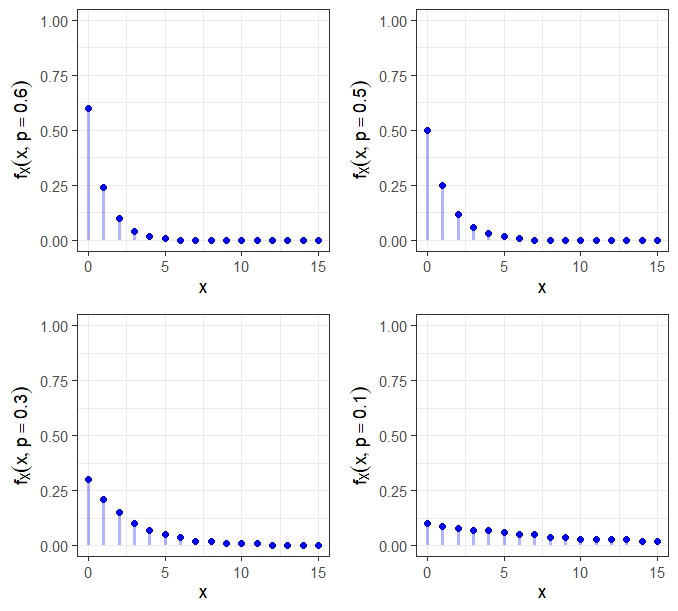
\includegraphics[scale=1]{Figuras/Geometrica.jpeg}
\caption{Función de masa de probabilidad Geométrica}
\end{figure}

\begin{theorem}
Si $X$ es una v.a con distribución geométrica dada por
\begin{equation*}
f(x;p)=p(1-p)^{x}I_{\{0,1,2,...\}}(x)
\end{equation*}%
\bigskip entonces%
\begin{eqnarray*}
E(X) &=&\frac{q}{p} \\
V(X) &=&\frac{q}{p^{2}} \\
m_{X}(t) &=&\frac{p}{1-qe^{t}}
\end{eqnarray*}
\end{theorem}

\textbf{Demostración}: Del Teorema de la Binomial negativa, se tiene el
resultado, para $r=1$.

\textbf{Observación}:
\begin{itemize}
\item La Binomial negativa es una generalización de la distribución geométrica, cuando se repiten los ensayos independientes, con probabilidad $p$, hasta obtener un número total de $r$ éxitos (pag. $95$, Casella, $1999$).

\item Existe al menos otra parametrización para la Binomial negativa.
\end{itemize}


\begin{definition}
La v.a $X$ tiene distribución Binomial negativa si su pmf está dada por 
\begin{equation*}
f(x,r,p)=\binom{x-1}{r-1}p^{r}(1-p)^{x-r}\text{, \ \ }x=r,r+1,...
\end{equation*}
\end{definition}

Note que $x-1$ son los primeros lanzamientos y $r-1$ son éxitos.
\textbf{Resultado:} Para una v.a $X$ con distribución Binomial negativa
dada por 
\begin{equation*}
f(x;r,p)=\binom{x-1}{r-1}p^{r}(1-p)^{x-r}\text{, \ \ }x=r,r+1,...
\end{equation*}%
se tiene que

\begin{eqnarray*}
E(X) &=&\frac{r}{p} \\
V(X) &=&\frac{rq}{p^{2}} \\
m(t) &=&\left( \frac{pe^{t}}{1-qe^{t}}\right) ^{r}
\end{eqnarray*}


\textbf{Tarea}: Demostrar el resultado anterior.

Note que para $r=1$ en la parametrización anterior, es decir,

\begin{equation*}
f(x;r,p)=\binom{x-1}{r-1}p^{r}(1-p)^{x-r}\text{, \ \ }x=r,r+1,...
\end{equation*}
se tiene que\ 
\begin{eqnarray*}
f(x;p) &=&\binom{x-1}{0}p(1-p)^{x-1} \\
&=&p(1-p)^{x-1}
\end{eqnarray*}
donde $x=1,2,...$

Es decir,
\begin{equation*}
f(x;p)=p(1-p)^{x-1}I_{\{1,2,3,..\}}(x)
\end{equation*}
es la parametrización de una variable aleatoria con distribución geométrica (Casella, $1999$).


\textbf{Resultado}: Si $X$ tiene distribución geométrica dada por
\begin{equation*}
f(x,r,p)=p(1-p)^{x-1}\text{, \ \ \ }x=1,2,..
\end{equation*}%
donde
\begin{eqnarray*}
E(X) &=&\frac{1}{p} \\
V(X) &=&\frac{q}{p^{2}} \\
m_{X}(t) &=&\frac{pe^{t}}{1-qe^{t}}
\end{eqnarray*}

\textbf{Tarea}: Demostrar el resultado anterior.


%%%%%%%%%%%%%%%%%%%%%%%%%%%%%%%%%%%%%%%%%%%%%%
\subsection{Logarítmica}

\begin{definition}
Una v.a $X$ con distribución logarítmica, está dada  por 
\begin{equation*}
f(x;p)=\frac{q^{x}}{-x\log _{e}(p)}I_{\{1,2,...\}}(x)
\end{equation*}%
donde $0<p<1$ y $q=1-p.$
\end{definition}

\begin{theorem}
 Si $X$ tiene distribución logarítmica, entonces
\begin{eqnarray*}
E(X) &=&\frac{q}{-p\log _{e}(p)} \\
&& \\
V(X) &=&\frac{q(q+\log _{e}(p))}{-(p\log _{e}(p))^{2}} \\
&& \\
m_{X}(t) &=&\frac{\log _{e}(1-qe^{t})}{\log _{e}(1-q)}
\end{eqnarray*}
\end{theorem}


\textbf{Tarea}: Deducir la $E(X)$ y la $V(X)$ a partir de la $m_{X}(t)$.


%%%%%%%%%%%%%%%%%%%%%%%%%%%%%%%%%%%%%%%%%%%%%%%%%%%%%%%%%%%%%%
\section{Distribuciones de probabilidad para v.a continuas}


%%%%%%%%%%%%%%%%%%%%%%%%%%%%%%%%%%%%%%%%%%%%%
\subsection{Uniforme continua}

\begin{definition}
Una v.a $X$ tiene distribución Uniforme en el intervalo $[a,b]$ si su pdf está dada por 
\begin{equation*}
f(x;a,b)=\frac{1}{b-a}I_{[a,b]}(x)
\end{equation*}%
donde $-\infty <a<b<\infty$.
\end{definition}

Note que:
\begin{itemize}
\item $b>a$

\item Cuando $X$ tiene distribución uniforme entonces se dice que $X\sim
U(a,b)$.
\end{itemize}


\begin{theorem}
 Si $X$ tiene distribución $U(a,b)$, entonces
\begin{eqnarray*}
E(X) &=&\frac{a+b}{2} \\
&& \\
V(X) &=&\frac{(b-a)^{2}}{12} \\
&& \\
m_{X}(t) &=&\frac{e^{bt}-e^{at}}{(b-a)t}
\end{eqnarray*}
\end{theorem} 

Demostración: 
\begin{eqnarray*}
E(X) &=&\int_{a}^{b}x\frac{1}{b-a}dx \\
&=&\frac{1}{b-a}\int_{a}^{b}xdx \\
&=&\frac{1}{b-a}\left. \frac{x^{2}}{2}\right\vert _{x=a}^{x=b} \\
&=&\frac{b^{2}-a^{2}}{2(b-a)} \\
&=&\frac{\left( b-a\right) \left( a+b\right) }{2(b-a)} \\
&=&\frac{a+b}{2}
\end{eqnarray*}

Por otra parte, 
\begin{eqnarray*}
E(X^{2}) &=&\int_{a}^{b}x^{2}\frac{1}{b-a}dx \\
&=&\frac{1}{b-a}\left. \frac{x^{3}}{3}\right\vert _{x=a}^{x=b} \\
&=&\frac{b^{3}-a^{3}}{3(b-a)} \\
&=&\frac{(b-a)(a^{2}+ab+b^{2})}{3(b-a)} \\
&=&\frac{a^{2}+ab+b^{2}}{3}
\end{eqnarray*}%
Luego 
\begin{eqnarray*}
V(X) &=&E(X^{2})-\left[ E(X)\right] ^{2} \\
&=&\frac{a^{2}+ab+b^{2}}{3}-\frac{\left( a+b\right) ^{2}}{4} \\
&=&\frac{4a^{2}+4ab+4b^{2}-3a^{2}-6ab-3b^{2}}{12} \\
&=&\frac{a^{2}+b^{2}-2ab}{12} \\
&=&\frac{(b-a)^{2}}{12}
\end{eqnarray*}

Por otra parte
\begin{eqnarray*}
m_{X}(t) &=&E(e^{tX}) \\
&=&\int_{a}^{b}\frac{e^{tx}}{b-a}dx \\
&=&\frac{1}{b-a}\int_{a}^{b}e^{tx}dx \\
&=&\frac{1}{t(b-a)}\int_{a}^{b}te^{tx}dx
\end{eqnarray*}
Sea $u=tx$ entonces 
\begin{equation*}
\frac{du}{dx}=t\text{, entonces }du=tdx
\end{equation*}
luego 
\begin{eqnarray*}
m_{X}(t) &=&\frac{1}{t(b-a)}\int_{a}^{b}e^{u}du \\
&=&\frac{1}{t(b-a)}\left. e^{tx}\right\vert _{a}^{b} \\
&=&\frac{e^{tb}-e^{ta}}{t(b-a)}
\end{eqnarray*}
Por lo tanto
\begin{equation*}
m_{X}(t)=\frac{e^{tb}-e^{ta}}{(b-a)t}
\end{equation*}

Note que:
\begin{itemize}
\item La pdf uniforme es constante en el intervalo $[a,b]$.

\item La cfd de una v.a $X$ uniforme, está dada por 
\begin{equation*}
F_{X}(x)=\frac{(x-a)}{b-a}I_{[a,b]}(x)+I_{(b,\infty )}(x)
\end{equation*}
\end{itemize}

%%%%%%%%%%%%%%%%%%%%%%%%%%%%%%%%
\subsection{Normal}

\begin{definition}
Una v.a $X$ tiene distribución normal si su pdf está dada por 
\begin{equation*}
f(x;\mu ,\sigma )=\frac{1}{\sqrt{2\pi \sigma ^{2}}}e^{-\frac{(x-\mu )^{2}}{
2\sigma ^{2}}}
\end{equation*}
donde $-\infty <\mu <\infty $, $\sigma >0;$ y $-\infty <x<\infty$.
\end{definition}

Observación:
\begin{itemize}
\item Generalmente se suele escribir como $X\sim N(\mu ,\sigma ^{2}).$
\end{itemize}

\begin{figure}[h!]
\centering
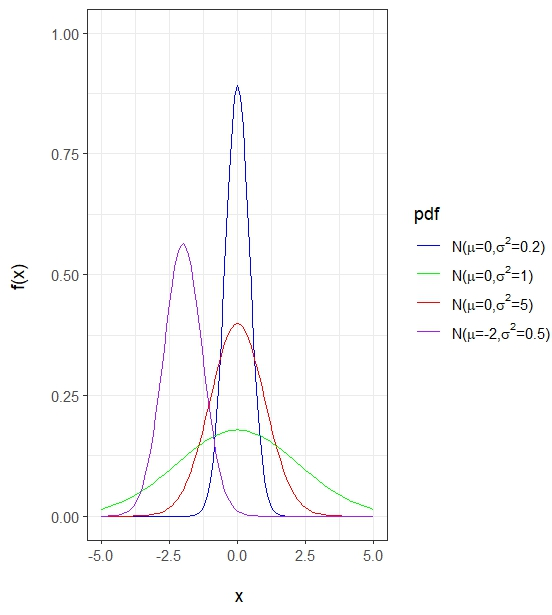
\includegraphics[scale=1]{Figuras/Normales.jpeg}
\caption{Distribuciones normales.}
\end{figure}

\begin{theorem}
Si $X$ tiene distribución $N(\mu ,\sigma ^{2})$, entonces
\begin{eqnarray*}
E(X) &=&\mu \\
V(X) &=&\sigma ^{2} \\
m_{X}(t) &=&e^{\mu t+\frac{(\sigma t)^{2}}{2}}
\end{eqnarray*}
\end{theorem}

Observaciones:
\begin{itemize}
\item La pdf de la v.a $X$, también se denota como: 
\begin{equation*}
\phi _{\mu,\sigma ^{2}}(x)=\frac{1}{\sqrt{2\pi \sigma ^{2}}}e^{-\frac{
(x-\mu )^{2}}{2\sigma ^{2}}}
\end{equation*}
\end{itemize}

\begin{itemize}
\item Si $\mu =0$ y $\sigma ^{2}=1$, entonces $X$ tiene distribución normal estándar:
\end{itemize}

\begin{equation*}
\phi _{\mu ,\sigma ^{2}}(x)=\phi (x)=\frac{1}{\sqrt{2\pi }}e^{-\frac{x^{2}}{2%
}}
\end{equation*}


\begin{itemize}
\item La función de distribución acumulativa (cdf) de una v.a $X$ con distribución $N(\mu ,\sigma ^{2})$, se denota con $\Phi _{\mu,\sigma ^{2}}(x)$, donde 
\begin{eqnarray*}
\Phi _{\mu ,\sigma ^{2}}(x) &=&F_{X}(x) \\
&=&P(X\leq x) \\
&=&\int_{-\infty }^{x}\frac{1}{\sqrt{2\pi \sigma ^{2}}}e^{-\frac{(u-\mu )^{2}%
}{2\sigma ^{2}}}du \\
&=&\int_{-\infty }^{x}\phi _{\mu ,\sigma ^{2}}(u)du
\end{eqnarray*}
\end{itemize}

Si $\mu =0$ y $\sigma ^{2}=1,$ entonces
\begin{equation*}
\Phi _{\mu ,\sigma ^{2}}(x)=\Phi (x)=\int_{-\infty }^{x}\phi (u)du
\end{equation*}

\begin{theorem}
Si $Z\sim N(0,1)$, entonces 
\begin{eqnarray*}
E(Z) &=&0 \\
V(Z) &=&1 \\
m_{Z}(t) &=&e^{t^{2}/2}
\end{eqnarray*}
\end{theorem} 

Demostración: 
\begin{eqnarray*}
E(Z) &=&\int_{-\infty }^{\infty }z\frac{1}{\sqrt{2\pi }}e^{-\frac{z^{2}}{2}
}dz \\
&=&\frac{1}{\sqrt{2\pi }}\int_{-\infty }^{\infty }ze^{-\frac{z^{2}}{2}}dz
\end{eqnarray*}

Sea $u=z^{2}/2$ entonces \ $du=zdz$

Luego
\begin{eqnarray*}
E(Z) &=&\frac{1}{\sqrt{2\pi }}\int_{-\infty }^{\infty }e^{-u}du \\
&=&\frac{1}{\sqrt{2\pi }}\left. e^{-\frac{z^{2}}{2}}\right\vert _{z=-\infty
}^{z=\infty } \\
&=&0
\end{eqnarray*}

Por otra parte 
\begin{eqnarray*}
E(Z^{2}) &=&\int_{-\infty }^{\infty }z^{2}\frac{1}{\sqrt{2\pi }}e^{-\frac{
z^{2}}{2}}dz \\
&=&\frac{1}{\sqrt{2\pi }}\int_{-\infty }^{\infty }zze^{-\frac{z^{2}}{2}}dz
\end{eqnarray*}

Considerando la integración por partes:
\begin{equation*}
\int uv^{\prime }=uv-\int u^{\prime }v
\end{equation*}
donde
\begin{eqnarray*}
u &=&z\text{ \ \ \ \ \ }v^{\prime }=ze^{-\frac{z^{2}}{2}} \\
du &=&dz\text{ \ \ \ }v=-e^{-\frac{z^{2}}{2}}
\end{eqnarray*}
Entonces%
\begin{eqnarray*}
E(Z^{2}) &=&\frac{1}{\sqrt{2\pi }}\int_{-\infty }^{\infty }zze^{-\frac{z^{2}
}{2}}dz \\
&=&\frac{1}{\sqrt{2\pi }}\left[ \left. -ze^{-\frac{z^{2}}{2}}\right\vert
_{z=-\infty }^{z=\infty }-\int_{-\infty }^{\infty }-e^{-\frac{z^{2}}{2}}dz
\right] \\
&=&\int_{-\infty }^{\infty }\frac{1}{\sqrt{2\pi }}e^{-\frac{z^{2}}{2}}dz%
\text{ \ \ \ //}Z\text{ es una pdf} \\
&=&1
\end{eqnarray*}
Luego 
\begin{eqnarray*}
V(Z) &=&E(Z^{2})-\left[ E(Z)\right] ^{2} \\
&=&1-0^{2} \\
&=&1
\end{eqnarray*}

Finalmente 
\begin{eqnarray*}
m_{Z}(t) &=&E(e^{tZ}) \\
&=&\int_{-\infty }^{\infty }e^{tz}\frac{1}{\sqrt{2\pi }}e^{-\frac{z^{2}}{2}
}dz \\
&=&\int_{-\infty }^{\infty }\frac{1}{\sqrt{2\pi }}e^{-\frac{z^{2}}{2}+tz}dz
\\
&=&\int_{-\infty }^{\infty }\frac{1}{\sqrt{2\pi }}e^{-\frac{1}{2}\left(
z^{2}-2tz+t^{2}-t^{2}\right) }dz \\
&=&\int_{-\infty }^{\infty }\frac{1}{\sqrt{2\pi }}e^{\frac{-1}{2}\left[
(z-t)^{2}-t^{2}\right] }dz \\
&=&\int_{-\infty }^{\infty }\frac{1}{\sqrt{2\pi }}e^{\frac{t^{2}}{2}}e^{%
\frac{-1}{2}(z-t)^{2}}dz \\
&=&e^{\frac{t^{2}}{2}}\int_{-\infty }^{\infty }\frac{1}{\sqrt{2\pi }}e^{%
\frac{-1}{2}(z-t)^{2}}dz\text{ //}Z\text{ es pdf} \\
&=&e^{\frac{t^{2}}{2}}
\end{eqnarray*}
Luego%
\begin{equation*}
m_{Z}(t)=e^{\frac{t^{2}}{2}}
\end{equation*}

\begin{teorem}
Si $X\sim N(\mu ,\sigma ^{2})$, entonces
\begin{eqnarray*}
E(X) &=&\mu \\
V(X) &=&\sigma ^{2} \\
m_{X}(t) &=&e^{\mu t+\frac{(\sigma t)^{2}}{2}}
\end{eqnarray*}
\end{teorem}
Demostración:

Sea 
\begin{equation*}
Z=\frac{X-\mu }{\sigma }
\end{equation*}

Note que $Z$ tiene distribución normal estándar, además

\begin{equation*}
X=\mu +\sigma Z
\end{equation*}
Luego%
\begin{eqnarray*}
E(X) &=&E(\mu +\sigma Z) \\
&=&\mu +\sigma E(Z)\text{ //Linealidad del operador} \\
&=&\mu +\sigma (0)\text{ //}Z\sim N(0,1)
\end{eqnarray*}%
i.e
\begin{equation*}
E(X)=\mu
\end{equation*}

Por otra parte 
\begin{eqnarray*}
E(X^{2}) &=&E\left[ (\mu +\sigma Z)^{2}\right] \\
&=&E\left[ \mu ^{2}+2\sigma Z+\sigma ^{2}Z^{2}\right] \\
&=&\mu ^{2}+2\sigma E(Z)+\sigma ^{2}E(Z^{2})\text{ //Linealidad del operador}
\\
&=&\mu ^{2}+\sigma ^{2}\text{ //}E(Z^{2})=1
\end{eqnarray*}

Entonces
\begin{equation*}
V(X)=\mu ^{2}+\sigma ^{2}-\mu ^{2}=\sigma ^{2}
\end{equation*}
Por lo tanto%
\begin{equation*}
V(X)=\sigma ^{2}
\end{equation*}

Finalmente%
\begin{eqnarray*}
m_{X}(t) &=&E(e^{tX}) \\
&=&E\left( e^{t(\mu +\sigma Z)}\right) \\
&=&e^{t\mu }E(e^{t\sigma Z})
\end{eqnarray*}
Como 
\begin{eqnarray*}
E(e^{t\sigma Z}) &=&\int_{-\infty }^{\infty }\frac{1}{\sqrt{2\pi }}e^{\frac{%
-1}{2}\left[ z^{2}-t\sigma z\right] }dz \\
&=&\int_{-\infty }^{\infty }\frac{1}{\sqrt{2\pi }}e^{\frac{-1}{2}\left[
(z-t\sigma )^{2}-t^{2}\sigma ^{2}\right] }dz \\
&=&\int_{-\infty }^{\infty }\frac{1}{\sqrt{2\pi }}e^{\frac{t^{2}\sigma ^{2}}{%
2}}e^{\frac{-1}{2}\left[ (z-t\sigma )^{2}\right] }dz \\
&=&e^{\frac{t^{2}\sigma ^{2}}{2}}\int_{-\infty }^{\infty }\frac{1}{\sqrt{%
2\pi }}e^{\frac{-1}{2}\left[ (z-t\sigma )^{2}\right] }dz \\
&=&e^{\frac{t^{2}\sigma ^{2}}{2}}
\end{eqnarray*}

Luego 
\begin{equation*}
m_{X}(t)=e^{t\mu +t^{2}\sigma ^{2}/2}
\end{equation*}

\begin{theorem}
Si $X\sim N(\mu ,\sigma ^{2})$ entonces
\begin{equation}
P(a<X<b)=\Phi \left( \frac{b-\mu }{\sigma }\right) -\Phi \left( \frac{a-\mu 
}{\sigma }\right)
\end{equation}
donde $a$, $b\in \mathbb{R}$.
\label{tem4}
\end{theorem}

Demostración:
\begin{equation*}
P(a<X<b)=\int_{a}^{b}\frac{1}{\sqrt{2\pi \sigma ^{2}}}e^{\frac{-1}{2}\left( 
\frac{x-\mu }{\sigma }\right) ^{2}}dx
\end{equation*}

Sea \ $z=\frac{x-\mu }{\sigma }$, entonces

\begin{equation*}
\begin{array}{lll}
P(a<X<b) & = & \int_{\frac{a-\mu }{\sigma }}^{\frac{b-\mu }{\sigma }}\frac{1
}{\sqrt{2\pi }}e^{\frac{-z^{2}}{2}}dx \\ 
& = & \int_{-\infty }^{\frac{b-\mu }{\sigma }}\frac{1}{\sqrt{2\pi }}e^{\frac{
-z^{2}}{2}}dx-\int_{-\infty }^{\frac{a-\mu }{\sigma }}\frac{1}{\sqrt{2\pi }}
e^{\frac{-z^{2}}{2}}dx \\ 
& = & \Phi \left( \frac{b-\mu }{\sigma }\right) -\Phi \left( \frac{a-\mu }{
\sigma }\right)
\end{array}
\end{equation*}
Por lo tanto 
\begin{equation*}
P(a<X<b)=\Phi \left( \frac{b-\mu }{\sigma }\right) -\Phi \left( \frac{a-\mu 
}{\sigma }\right)
\end{equation*}


La distribución normal tiene las siguientes características:

\begin{itemize}
    \item Simetría: Es simétrica alrededor de la media, lo que significa que las colas izquierda y derecha de la distribución son idénticas.
    \item Unimodal: Tiene un solo pico en la media.
    \item Forma de Campana: La función de densidad de probabilidad forma una curva en forma de campana.
    \item  Aproximadamente el 68\% de los datos caen dentro de una desviación estándar de la media, el 95\% dentro de dos desviaciones estándar y el 99.7\% dentro de tres desviaciones estándar.

\end{itemize}



%%%%%%%%%%%%%%%%%%%%%%%%%%%%%%%%%%%%%%%%%
\subsubsection{Resolución de problemas}

Para una variable aleatoria $X$, con distribución normal, $\mu=100$ y $sd=10$, calcular
$$
P(90 \leq X \leq 115)
$$
Esta probabilidad se puede calcular:
\begin{itemize}
    \item Integrando la pdf de la normal con $\mu=100$ y $sd=10$.
    \item Usando el Teorema (\ref{tem4}).
    \item Usando R.
\end{itemize}

\begin{figure}[h!]
\centering
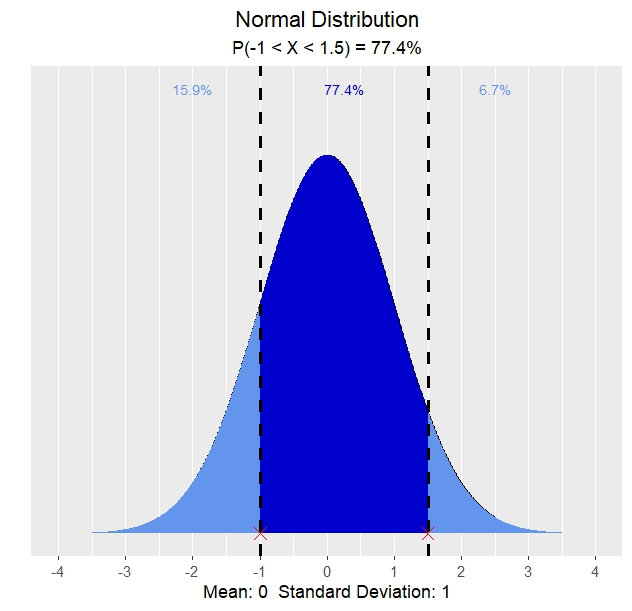
\includegraphics[scale=0.8]{Figuras/Normal_prob.jpeg}
\caption{Normal estándar.}
\end{figure}

Para una variable aleatoria $X$, con distribución normal, $\mu=100$ y $sd=10$, calcular
$$
P(X \leq 115)
$$
\begin{figure}[h!]
\centering
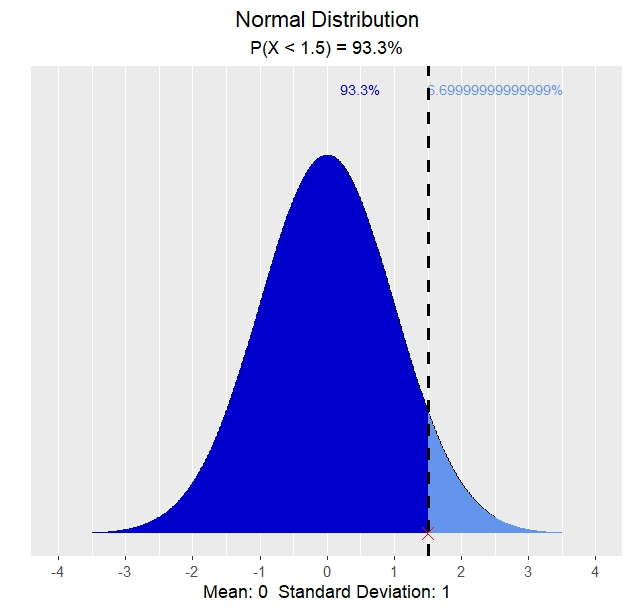
\includegraphics[scale=0.8]{Figuras/Normal2_prob.jpeg}
\caption{Normal estándar.}
\end{figure}


%%%%%%%%%%%%%%%%%%%%%%%%%%%%%%%%%%%%%%%%%
\subsubsection{Práctica con R}

Funciones para la distribución normal:
\begin{itemize}
\item dnorm(x, mean, sd), calcula $f(x)$
\item pnorm(q, mean, sd, lower.tail=TRUE),  calcula $P(X<q)$
\item qnorm(p, mean, sd, lower.tail=TRUE),  calcula $q$ tal que $P(X<q) = p$
\item rnorm(n, mean, sd), genera números aleatorios
\end{itemize}

\vspace{5mm}
Paquetes
\begin{lstlisting}
    library(vistributions)
    library(devtools)
\end{lstlisting}
\vspace{5mm}
Cálculo de 
$$
P(90 \leq X \leq 115)
$$
\begin{lstlisting}
      mu<-100
      sd<-10
      z1<-(90-mu)/sd
      z2<-(115-mu)/sd
      vdist_normal_prob(c(z1, z2),
                        mean =0, 
                        sd = 1,
                        type = 'both')
\end{lstlisting}

\vspace{5mm}
Cálculo de 
$$
P(90 \leq X \leq 115)
$$
\begin{lstlisting}
      p_sup <- pnorm(q=115, mean=100, sd=10)
      p_inf <- pnorm(q=90, mean=100, sd=10)
      p_sup - p_inf
\end{lstlisting}
\vspace{5mm}

Cálculo de
$$
P(X \leq 115)
$$
\begin{lstlisting}
      mu<-100
      sd<-10
      z2<-(115-mu)/sd;z2

      vdist_normal_prob(z2,
                        mean = 0,
                        sd = 1,
                        type ="lower")
\end{lstlisting}

\vspace{5mm}
Cálculo de
$$
P(X \leq 115)
$$
\begin{lstlisting}
      # pnorm() entrega la probabilidad de cola a izquierda.

      pnorm(q=115, mean=100, sd=10)
\end{lstlisting}

\vspace{5mm}
Cálculo de
$$
P(X \leq 115)
$$

\begin{lstlisting}
       mu<-100
       sd<-10
       var.x<-sd*sd

       pdf_normal <- function(x) 
             {
              (1/sqrt(2*pi*var.x))*exp(-(x-mu)^2/(2*var.x))
             }



        integrate(pdf_normal , lower=0, upper=115)
\end{lstlisting}

%%%%%%%%%%%%%%%%%%%%%%%%%%%%%%%%%%%%%%%%%
\subsection{Exponencial}

\begin{definition}
Una v.a $X$ tiene distribución Exponencial si su función densidad está dada por 
\begin{equation*}
f_{X}(x;\lambda )=\lambda e^{-\lambda x}I_{[0,\infty )}(x)
\end{equation*}
con $\lambda >0$. // $X\sim Exp(\lambda )$
\end{definition}

\begin{figure}[h!]
\centering
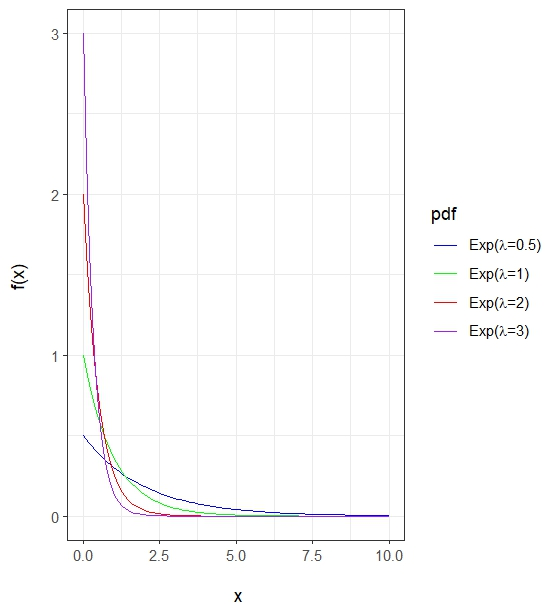
\includegraphics[scale=1]{Figuras/Exponenciales.jpeg}
\caption{Distribuciones exponenciales.}
\end{figure}


\begin{theorem}
 Si $X$ tiene distribución $Exp(\lambda)$, entonces
\begin{eqnarray*}
E(X) &=&\frac{1}{\lambda } \\
V(X) &=&\frac{1}{\lambda ^{2}} \\
m_{X}(t) &=&\frac{\lambda }{\lambda -t}\text{, }\lambda >t
\end{eqnarray*}
\end{theorem}

Demostración:
\begin{eqnarray*}
E(X) &=&\int_{-\infty }^{\infty }xf_{X}(x)dx \\
&=&\int_{0}^{\infty }x\lambda e^{-\lambda x}dx \\
&=&\lambda \int_{0}^{\infty }xe^{-\lambda x}dx
\end{eqnarray*}

Se efectúa una integración por partes: $\int uv^{\prime }=uv-\int u^{\prime }v$
\begin{eqnarray*}
u &=&x\text{ \ \ \ \ \ \ \ \ \ \ \ \ }du=dx \\
v^{\prime } &=&e^{-\lambda x}dx\text{ \ \ \ }v=-\frac{e^{-\lambda x}}{%
\lambda }
\end{eqnarray*}%
luego
\begin{eqnarray*}
E(X) &=&\lambda \left[ \left. \left( x\frac{\left( -e^{-\lambda x}\right) }{%
\lambda }\right) \right\vert _{0}^{\infty }-\int_{0}^{\infty }-\frac{%
e^{-\lambda x}}{\lambda }dx\right] \\
&=&\int_{0}^{\infty }e^{-\lambda x}dx
\end{eqnarray*}
sea 
\begin{equation*}
u=-\lambda x\text{ \ }du=-\lambda dx
\end{equation*}
\begin{eqnarray*}
E(X) &=&\int_{0}^{\infty }e^{-\lambda x}dx \\
&=&-\frac{1}{\lambda }\int_{0}^{\infty }e^{u}du \\
&=&-\frac{1}{\lambda }\left. e^{u}\right\vert _{0}^{\infty } \\
&=&-\frac{1}{\lambda }\left( 0-1\right) \\
&=&\frac{1}{\lambda }
\end{eqnarray*}

i.e
\begin{equation*}
E(X)=\frac{1}{\lambda }
\end{equation*}

Por otra parte, como 
\begin{equation*}
V(X)=E(X^{2})-\left[ E(X)\right] ^{2}
\end{equation*}

Entonces
\begin{eqnarray*}
E(X^{2}) &=&\int_{-\infty }^{\infty }x^{2}f_{X}(x)dx \\
&=&\int_{0}^{\infty }x^{2}\lambda e^{-\lambda x}dx \\
&=&\lambda \int_{0}^{\infty }x^{2}e^{-\lambda x}dx
\end{eqnarray*}

Realizando una integración por partes: $\int uv^{\prime }=uv-\int u^{\prime }v$

\begin{eqnarray*}
u &=&x^{2}\text{ \ \ \ \ \ \ \ \ \ \ \ \ }\frac{du}{dx}=2x \\
dv &=&e^{-\lambda x}dx\text{ \ \ \ \ \ \ \ \ }v=-\frac{e^{-\lambda x}}{\lambda}
\end{eqnarray*}
Entonces
\begin{eqnarray*}
E(X^{2}) &=&\left. \left( -\lambda x^{2}\frac{e^{-\lambda x}}{\lambda }
\right) \right\vert _{0}^{\infty }-\lambda \int_{0}^{\infty }-\frac{
e^{-\lambda x}}{\lambda }2xdx \\
&=&\int_{0}^{\infty }e^{-\lambda x}2xdx \\
&=&2\int_{0}^{\infty }xe^{-\lambda x}dx \\
&=&\frac{2}{\lambda }\int_{0}^{\infty }\lambda xe^{-\lambda x}dx
\end{eqnarray*}

Note que
\begin{equation*}
\int_{0}^{\infty }\lambda xe^{-\lambda x}dx=E(X)=1/\lambda
\end{equation*}

Entonces, sustituyendo
\begin{eqnarray*}
E(X^{2}) &=&\frac{2}{\lambda }\cdot \frac{1}{\lambda } \\
&=&\frac{2}{\lambda ^{2}}
\end{eqnarray*}

Luego 
\begin{eqnarray*}
V(X) &=&E(X^{2})-\left[ E(X)\right] ^{2} \\
&=&\frac{2}{\lambda ^{2}}-\frac{1}{\lambda ^{2}} \\
&=&\frac{1}{\lambda ^{2}}
\end{eqnarray*}

Finalmente 
\begin{eqnarray*}
m_{X}(t) &=&E(e^{tX}) \\
&=&\int_{0}^{\infty }e^{tx}\lambda e^{-\lambda x}dx \\
&=&\int_{0}^{\infty }\lambda e^{tx}e^{-\lambda x}dx \\
&=&\lambda \int_{0}^{\infty }e^{-x(\lambda -t)}dx \\
&=&\frac{\lambda }{\lambda -t}\int_{0}^{\infty }\left( \lambda -t\right)
e^{-x(\lambda -t)}dx\text{ // }\lambda -t>0, \\
&=&\frac{\lambda }{\lambda -t}
\end{eqnarray*}
Por lo tanto 
\begin{equation*}
m_{X}(t)=\frac{\lambda }{\lambda -t}.
\end{equation*}

Una segunda parametrización para la pdf exponencial (Casella, 1990), está dada por
\begin{equation*}
f(x)=\frac{1}{\lambda }e^{-\frac{x}{\lambda }}I_{(0,\infty )}(x)
\end{equation*}%
donde $\lambda >0.$ En este caso 
\begin{eqnarray*}
E(X) &=&\lambda \\
V(X) &=&\lambda ^{2} \\
m_{X}(t) &=&\frac{1}{1-\lambda t}\text{, }\frac{1}{\lambda }>t
\end{eqnarray*}

\textbf{Tarea}: Demostrarlo.



%%%%%%%%%%%%%%%%%%%%%%%%%%%%%%%%%%%
\subsection{Gamma}


\begin{definition}
Una v.a $X$ tiene distribución Gamma($r,\lambda $) si su pdf está dada por 
\begin{equation*}
f(x;r,\lambda )=\frac{\lambda }{\Gamma (r)}\left( \lambda x\right)
^{r-1}e^{-\lambda x}I_{[0,\infty )}(x)
\end{equation*}
con $r,\lambda >0.$
\end{definition}

\begin{figure}[h!]
\centering
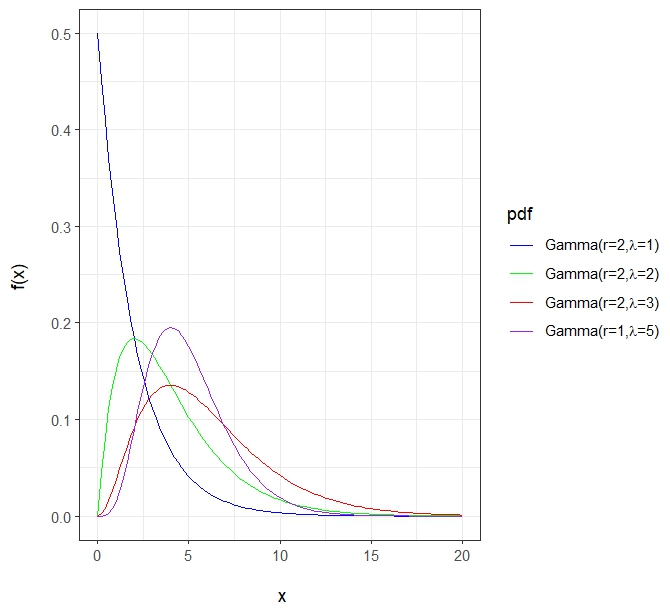
\includegraphics[scale=1]{Figuras/Gammas.jpeg}
\caption{Distribuciones Gammas.}
\end{figure}

\begin{theorem}
Si $X$ tiene distribución Gamma($r,\lambda$), entonces
\begin{eqnarray*}
E(X) &=&\frac{r}{\lambda } \\
V(X) &=&\frac{r}{\lambda ^{2}} \\
m_{X}(t) &=&\left( \frac{\lambda }{\lambda -t}\right) ^{r}\text{, \ }t\leq
\lambda
\end{eqnarray*}
\end{theorem}


Demostración
\begin{eqnarray*}
E(X) &=&\int_{0}^{\infty }x\frac{\lambda }{\Gamma (r)}\left( \lambda
x\right) ^{r-1}e^{-\lambda x}dx \\
&=&\int_{0}^{\infty }x\frac{\lambda }{\Gamma (r)}\lambda
^{r-1}x^{r-1}e^{-\lambda x}dx \\
&=&\int_{0}^{\infty }\frac{\lambda ^{r}}{\Gamma (r)}x^{r}e^{-\lambda x}dx \\
&=&\frac{\lambda ^{r}}{\Gamma (r)}\int_{0}^{\infty }x^{r}e^{-\lambda x}dx
\end{eqnarray*}

Realizando integración por partes: $\int uv^{\prime }=uv-\int u^{\prime}v$
\begin{equation*}
\begin{array}{ccc}
u=x^{r} &  & v^{\prime }=e^{-\lambda x} \\ 
\frac{du}{dx}=rx^{r-1} &  & v=\frac{-e^{-\lambda x}}{\lambda }
\end{array}
\end{equation*}

Entonces
\begin{eqnarray*}
E(X) &=&\frac{\lambda ^{r}}{\Gamma (r)}\int_{0}^{\infty }x^{r}e^{-\lambda
x}dx \\
&=&\left. \frac{\lambda ^{r}}{\Gamma (r)}x^{r}\left( -\frac{e^{-\lambda x}}{%
\lambda }\right) \right\vert _{x=0}^{x=\infty }-\frac{\lambda ^{r}}{\Gamma
(r)}\int_{0}^{\infty }rx^{r-1}\left( \frac{-e^{-\lambda x}}{\lambda }\right)
dx \\
&=&\int_{0}^{\infty }\frac{\lambda }{\Gamma (r)}\lambda ^{r-1}rx^{r-1}\left( 
\frac{e^{-\lambda x}}{\lambda }\right) dx \\
&=&\frac{r}{\lambda }\int_{0}^{\infty }\frac{\lambda }{\Gamma (r)}\lambda
^{r-1}x^{r-1}e^{-\lambda x}dx \\
&=&\frac{r}{\lambda }\int_{0}^{\infty }\frac{\lambda }{\Gamma (r)}(\lambda
x)^{r-1}e^{-\lambda x}dx\text{ \ // pdf gamma} \\
&=&\frac{r}{\lambda }
\end{eqnarray*}

Luego
\begin{equation*}
E(X)=\frac{r}{\lambda }
\end{equation*}

Por otra, parte, 
\begin{equation*}
V(X)=E(X^{2})-[E(X)]^{2}
\end{equation*}

entonces
\begin{eqnarray*}
E(X^{2}) &=&\int_{0}^{\infty }x^{2}\frac{\lambda }{\Gamma (r)}\lambda
^{r-1}x^{r-1}e^{-\lambda x}dx \\
&=&\int_{0}^{\infty }\frac{\lambda }{\Gamma (r)}\lambda
^{r-1}x^{r+1}e^{-\lambda x}dx \\
&=&\int_{0}^{\infty }\frac{\lambda ^{r}}{\Gamma (r)}x^{r+1}e^{-\lambda x}dx
\\
&=&\frac{\lambda ^{r}}{\Gamma (r)}\int_{0}^{\infty }x^{r+1}e^{-\lambda x}dx
\end{eqnarray*}

Realizando integración por partes: $\int uv^{\prime }=uv-\int u^{\prime}v$

$u=x^{r+1}$,  $v^{\prime }=e^{-\lambda x}$

$\frac{du}{dx}=(r+1)x^{r}$  $v=\frac{-e^{-\lambda x}}{\lambda}$

Entonces
\begin{eqnarray*}
E(X^{2}) &=&\frac{\lambda ^{r}}{\Gamma (r)}\int_{0}^{\infty
}x^{r+1}e^{-\lambda x}dx \\
&=&\left. \frac{\lambda ^{r}}{\Gamma (r)}x^{r+1}\left( \frac{-e^{-\lambda x}%
}{\lambda }\right) \right\vert _{x=0}^{x=\infty }-\frac{\lambda ^{r}}{\Gamma
(r)}\int_{0}^{\infty }(r+1)x^{r}\left( \frac{-e^{-\lambda x}}{\lambda }%
\right) dx \\
&=&\frac{\lambda ^{r}}{\Gamma (r)}\int_{0}^{\infty }(r+1)x^{r}\frac{%
e^{-\lambda x}}{\lambda }dx \\
&=&\frac{(r+1)}{\lambda }\int_{0}^{\infty }\frac{\lambda ^{r}}{\Gamma (r)}%
x^{r}e^{-\lambda x}dx \\
&=&\frac{(r+1)}{\lambda }\int_{0}^{\infty }\frac{\lambda }{\Gamma (r)}%
\lambda ^{r-1}x^{r}e^{-\lambda x}dx
\end{eqnarray*}
Note que 
\begin{equation*}
E(X)=\int_{0}^{\infty }\frac{\lambda }{\Gamma (r)}\lambda
^{r-1}x^{r}e^{-\lambda x}dx=\frac{r}{\lambda }
\end{equation*}
Sustituyendo%
\begin{eqnarray*}
E(X^{2}) &=&\frac{(r+1)}{\lambda }\cdot \frac{r}{\lambda } \\
&=&\frac{r(r+1)}{\lambda ^{2}}
\end{eqnarray*}

Entonces
\begin{eqnarray*}
V(X) &=&E(X^{2})-\left[ E(X)\right] ^{2} \\
&=&\frac{r^{2}+r}{\lambda ^{2}}-\frac{r^{2}}{\lambda ^{2}}\text{ } \\
&=&\frac{r}{\lambda ^{2}}
\end{eqnarray*}

Por otra parte 
\begin{eqnarray*}
m_{X}(t) &=&E(e^{tX}) \\
&=&\int_{0}^{\infty }e^{tx}\frac{\lambda }{\Gamma (r)}\left( \lambda
x\right) ^{r-1}e^{-\lambda x}dx \\
&=&\int_{0}^{\infty }\frac{\lambda }{\Gamma (r)}(\lambda
x)^{r-1}e^{-(\lambda -t)x}dx \\
&=&\int_{0}^{\infty }\frac{\lambda }{\Gamma (r)}\lambda
^{r-1}x^{r-1}e^{-(\lambda -t)x}dx \\
&=&\int_{0}^{\infty }\frac{\lambda ^{r}}{\Gamma (r)}x^{r-1}e^{-(\lambda
-t)x}dx \\
&=&\frac{\lambda ^{r}}{(\lambda -t)^{r}}\int_{0}^{\infty }\frac{(\lambda
-t)^{r}}{\Gamma (r)}x^{r-1}e^{-(\lambda -t)x}dx \\
&=&=\frac{\lambda ^{r}}{(\lambda -t)^{r}}\int_{0}^{\infty }\frac{(\lambda -t)%
}{\Gamma (r)}(\lambda -t)^{r-1}x^{r-1}e^{-(\lambda -t)x}dx \\
&=&\frac{\lambda ^{r}}{(\lambda -t)^{r}}\int_{0}^{\infty }\frac{(\lambda -t)%
}{\Gamma (r)}\left[ (\lambda -t)x\right] ^{r-1}e^{-(\lambda -t)x}dx\text{ }
\end{eqnarray*}

Note que 
\begin{equation*}
\int_{0}^{\infty }\frac{(\lambda -t)}{\Gamma (r)}\left[ (\lambda -t)x\right]
^{r-1}e^{-(\lambda -t)x}dx
\end{equation*}%
es la pdf de una Gamma($r,(\lambda -t)$), donde $\lambda -t>0$ ($\lambda >0,$
$\left\vert h\right\vert <t,$ $h>0$) es decir $\lambda >t.$ Entonces 
\begin{equation*}
\int_{0}^{\infty }\frac{(\lambda -t)}{\Gamma (r)}\left[ (\lambda -t)x\right]
^{r-1}e^{-(\lambda -t)x}dx=1
\end{equation*}

Luego
\begin{equation*}
m_{X}(t)=\frac{\lambda ^{r}}{(\lambda -t)^{r}}=\left( \frac{\lambda }{%
\lambda -t}\right) ^{r}\text{, \ }t<\lambda
\end{equation*}

Por lo tanto, 
\begin{equation*}
m_{X}(t)=\left( \frac{\lambda }{\lambda -t}\right) ^{r}\text{, \ }t<\lambda
\end{equation*}

Una segunda parametrización para la pdf de una Gamma, está dada por (Casella, $1990$) 
\begin{equation*}
f(x,r,\lambda )=\frac{1}{\Gamma (r)\lambda ^{r}}x^{r-1}e^{-x/\lambda
}I_{(0,\infty )}(x)
\end{equation*}

Donde
\begin{eqnarray*}
E(X) &=&r\lambda \\
V(X) &=&r\lambda ^{2} \\
m_{X}(t) &=&\left( \frac{1}{1-\lambda t}\right) ^{r}\text{, }t<\frac{1}{%
\lambda }
\end{eqnarray*}


\textbf{Tarea}: Demostrarlo.

%%%%%%%%%%%%%%%%%%%%%%%%%%%%%%%%%%
\subsection{Chi cuadrada}

\begin{definition}
La  pdf de la $\chi^2$ está dada por
$$
f(x)=\frac{1}{\Gamma(k/2)}\left(\frac{1}{2}\right)^{k/2}x^{k/2-1}e^{-(1/2)x}I_{(0,\infty)}(x)
$$    
$k=1,2,...$, $0\leq x\leq \infty $
\end{definition}

\begin{figure}[h!]
\centering
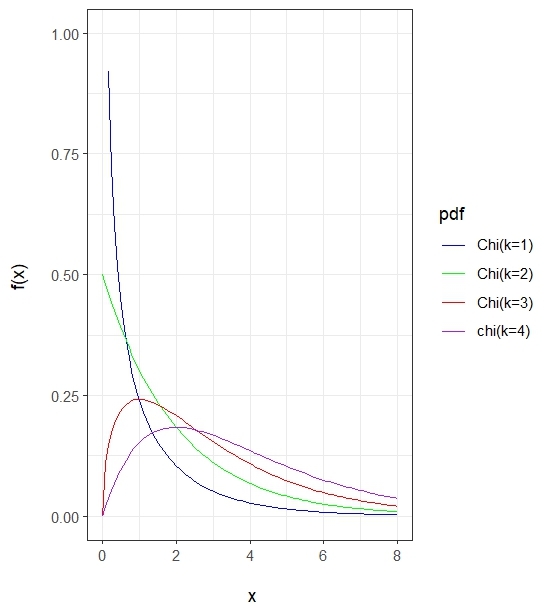
\includegraphics[scale=1]{Figuras/Chi_cuadradas.jpeg}
\caption{Distribución Chi cuadrada.}
\end{figure}

\begin{theorem}
Si $X$ tiene distribución $\chi^2$ con $k$ grados de libertad, entonces

\begin{eqnarray*}
E(X) &=&k \\
V(X) &=&2k \\
m_{X}(t) &=&\left( \frac{1 }{1 -2t}\right)^{k/2}\text{, \ }t\leq 1/2
\end{eqnarray*}
\end{theorem}


%%%%%%%%%%%%%%%%%%%%%%%%%%%%%%%%%%
\subsection{Beta}

\begin{definition}
Una v.a $X$ tiene distribución $Beta(a,b)$ si su función densidad está dada por 
\begin{equation*}
f(x;a,b)=\frac{1}{B(a,b)}x^{a-1}(1-x)^{b-1}I_{(0,1)}(x)
\end{equation*}
con $a,b>0.$ \ //$X\sim Beta(a,b)$
\end{definition}

\begin{figure}[h!]
\centering
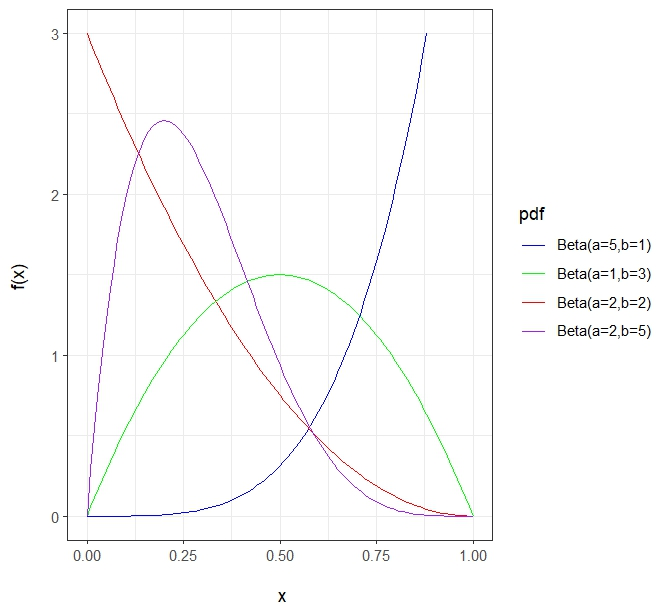
\includegraphics[scale=1]{Figuras/Betas.jpeg}
\caption{Distribuciones Betas.}
\end{figure}

\begin{definition}
A la función
\begin{equation*}
B(a,b)=\int_{0}^{1}x^{a-1}(1-x)^{b-1}dx
\end{equation*}
se le llama función beta, y tiene las siguientes propiedades: 
\begin{eqnarray*}
B(a,b) &=&\frac{\Gamma (a)\Gamma (b)}{\Gamma (a+b)} \\
B(a,b) &=&B(b,a)
\end{eqnarray*}
\end{definition}

\begin{figure}[h!]
\centering
\includegraphics[scale=1]{Figuras/Beta.jpeg}
\caption{Distribución Beta.}
\end{figure}


\begin{theorem}
Si $X$ tiene distribución Beta($a$, $b$), entonces
\begin{eqnarray*}
E(X) &=&\frac{a}{a+b} \\
V(X) &=&\frac{ab}{(a+b+1)(a+b)^{2}} \\
m_{X}(t) &=&1+\sum_{k=1}^{\infty }\frac{t^{k}}{k!}\left(
\prod\limits_{r=0}^{k-1}\frac{a+r}{a+b+r}\right)
\end{eqnarray*}
\end{theorem}

Demostración:
\begin{eqnarray*}
E(X^{k}) &=&\int_{0}^{1}x^{k}\frac{1}{B(a,b)}x^{a-1}(1-x)^{b-1}dx \\
&=&\frac{1}{B(a,b)}\int_{0}^{1}x^{k+a-1}(1-x)^{b-1}dx\text{ \ }//\text{Def.}
\\
&=&\frac{B(k+a,b)}{B(a,b)} \\
&=&\frac{\Gamma (k+a)\Gamma (b)/\Gamma (k+a+b)}{\Gamma (a)\Gamma (b)/\Gamma
(a+b)} \\
&=&\frac{\Gamma (a+b)\Gamma (k+a)\Gamma (b)}{\Gamma (k+a+b)\Gamma (a)\Gamma
(b)} \\
&=&\frac{\Gamma (a+b)\Gamma (k+a)}{\Gamma (a)\Gamma (k+a+b)}
\end{eqnarray*}

Luego 
\begin{equation*}
E(X^{k})=\frac{\Gamma (a+b)\Gamma (k+a)}{\Gamma (a)\Gamma (k+a+b)}
\end{equation*}


Por otra parte (Mood, pag. $534$),

\begin{equation*}
\Gamma (r)=\int_{0}^{\infty }x^{r-1}e^{-x}dx
\end{equation*}%
entonces 
\begin{equation*}
\Gamma (r+1)=\int_{0}^{\infty }x^{r}e^{-x}dx
\end{equation*}

Note que 
\begin{equation*}
\Gamma (r+1)=r\Gamma (r)
\end{equation*}

Lo cual se puede justificar de la siguiente manera: Realizando integración por partes: $\int uv^{\prime }=uv-\int u^{\prime }v$

$u=x^{r}$ \ \ \ \ \ \ \ \ \ \ $v^{\prime }=e^{-x}$

$\frac{du}{dx}=rx^{r-1}$ \ \ \ $v=-e^{-x}$

\begin{eqnarray*}
\Gamma (r+1) &=&\left. x^{r}(-e^{-x})\right\vert _{0}^{\infty
}-\int_{0}^{\infty }rx^{r-1}(-e^{-x})dx \\
&=&r\int_{0}^{\infty }x^{r-1}e^{-x}dx\text{ \ //}\Gamma (t)=\int_{0}^{\infty
}x^{t-1}e^{-x}dx \\
&=&r\Gamma (r)
\end{eqnarray*}
es decir 
\begin{equation*}
\Gamma (r+1)=r\Gamma (r)
\end{equation*}


Para $k=1$ en 
\begin{equation*}
E(X^{k})=\frac{\Gamma (a+b)\Gamma (k+a)}{\Gamma (a)\Gamma (k+a+b)}
\end{equation*}%
se tiene que

\begin{eqnarray*}
E(X) &=&\frac{\Gamma (a+b)\Gamma (1+a)}{\Gamma (a)\Gamma (1+a+b)}\text{ \ // 
}\Gamma (r+1)=r\Gamma (r) \\
&=&\frac{\Gamma (a+b)a\Gamma (a)}{\Gamma (a)(a+b)\Gamma (a+b)} \\
&=&\frac{a}{a+b}
\end{eqnarray*}

Entonces 
\begin{equation*}
E(X)=\frac{a}{a+b}
\end{equation*}

Para $k=2$ en
\begin{equation*}
E(X^{k})=\frac{\Gamma (a+b)\Gamma (k+a)}{\Gamma (a)\Gamma (k+a+b)}
\end{equation*}

se tiene lo siguiente
\begin{eqnarray*}
E(X^{2}) &=&\frac{\Gamma (a+b)\Gamma (2+a)}{\Gamma (a)\Gamma (2+a+b)} \\
&=&\frac{\Gamma (a+b)\Gamma (1+(1+a))}{\Gamma (a)\Gamma (1+(1+a+b))}\text{ \
\ \ // }\Gamma (r+1)=r\Gamma (r) \\
&=&\frac{\Gamma (a+b)(a+1)\Gamma (a+1)}{\Gamma (a)(1+a+b)\Gamma (1+a+b)}%
\text{ \ \ // }\Gamma (r+1)=r\Gamma (r) \\
&=&\frac{\Gamma (a+b)(a+1)a\Gamma (a)}{\Gamma (a)(1+a+b)(a+b)\Gamma (a+b)}%
\text{ } \\
&=&\frac{a(a+1)}{(a+b)(1+a+b)}
\end{eqnarray*}

Luego 
\begin{eqnarray*}
V(X) &=&E(X^{2})-[E(X)]^{2} \\
&=&\frac{a(a+1)}{(a+b)(1+a+b)}-\frac{a^{2}}{(a+b)^{2}} \\
&=&\frac{(a+b)(a^{2}+a)-a^{2}(1+a+b)}{(1+a+b)(a+b)^{2}} \\
&=&\frac{a^{3}+ab^{2}+a^{2}+ab-a^{2}-a^{3}-a^{2}b}{(1+a+b)(a+b)^{2}} \\
&=&\frac{ab}{(1+a+b)(a+b)^{2}}
\end{eqnarray*}
es decir,
\begin{equation*}
V(X)=\frac{ab}{(1+a+b)(a+b)^{2}}
\end{equation*}

Finalmente 
\begin{eqnarray*}
m_{X}(t) &=&E(e^{tX}) \\
&=&\int_{0}^{1}\frac{e^{tx}}{B(a,b)}x^{a-1}(1-x)^{b-1}dx \\
&=&\frac{1}{B(a,b)}\int_{0}^{1}\sum_{k=0}^{\infty }\frac{(tx)^{k}}{k!}%
x^{a-1}(1-x)^{b-1}dx \\
&=&\frac{1}{B(a,b)}\int_{0}^{1}\sum_{k=0}^{\infty }\frac{t^{k}x^{k}}{k!}%
x^{a-1}(1-x)^{b-1}dx \\
&=&\frac{1}{B(a,b)}\sum_{k=0}^{\infty }\frac{t^{k}}{k!}%
\int_{0}^{1}x^{k}x^{a-1}(1-x)^{b-1}dx \\
&=&\frac{1}{B(a,b)}\sum_{k=0}^{\infty }\frac{t^{k}}{k!}\int_{0}^{1}\frac{%
B(a+k,b)}{B(a+k,b)}x^{k+a-1}(1-x)^{b-1}dx\text{ } \\
&=&\frac{1}{B(a,b)}\sum_{k=0}^{\infty }\frac{t^{k}}{k!}B(a+k,b)\int_{0}^{1}%
\frac{1}{B(a+k,b)}x^{k+a-1}(1-x)^{b-1}dx\text{ //pdf} \\
&=&\sum_{k=0}^{\infty }\frac{t^{k}}{k!}\frac{B(a+k,b)}{B(a,b)} \\
&=&\sum_{k=0}^{\infty }\frac{t^{k}}{k!}\left[ \left. \frac{\Gamma
(a+k)\Gamma (b)}{\Gamma (a+b+k)}\right/ \frac{\Gamma (a)\Gamma (b)}{\Gamma
(a+b)}\right] \text{ \ \ //}B(a,b)=\frac{\Gamma (a)\Gamma (b)}{\Gamma (a+b)}
\\
&=&\sum_{k=0}^{\infty }\frac{t^{k}}{k!}\left[ \frac{\Gamma (a+b)\Gamma
(a+k)\Gamma (b)}{\Gamma (a+b+k)\Gamma (a)\Gamma (b)}\right] \\
&=&\sum_{k=0}^{\infty }\frac{t^{k}}{k!}\left[ \frac{\Gamma (a+b)\Gamma (a+k)%
}{\Gamma (a)\Gamma (a+b+k)}\right] \text{ } \\
&=&1+\sum_{k=1}^{\infty }\frac{t^{k}}{k!}\left[ \frac{\Gamma (a+b)\Gamma
(a+k)}{\Gamma (a)\Gamma (a+b+k)}\right] \\
&=&1+\sum_{k=1}^{\infty }\frac{t^{k}}{k!}\left[ \frac{\Gamma (a+b)\Gamma
(a)\prod\limits_{r=0}^{k-1}(a+r)}{\Gamma (a)\Gamma
(a+b)\prod\limits_{r=0}^{k-1}(a+b+r)}\right] \text{ } \\
&=&1+\sum_{k=1}^{\infty }\frac{t^{k}}{k!}\left[ \prod\limits_{r=0}^{k-1}%
\frac{a+r}{a+b+r}\right] \text{ }
\end{eqnarray*}

Luego
\begin{equation*}
m_{X}(t)=1+\sum_{k=1}^{\infty }\frac{t^{k}}{k!}\left[ \prod%
\limits_{r=0}^{k-1}\frac{a+r}{a+b+r}\right] \text{ }
\end{equation*}


%%%%%%%%%%%%%%%%%%%%%%%%%%%%%%%%%%
\subsection{Cauchy}

\begin{definition}
Una v.a $X$ tiene distribución Cauchy si su función densidad está dada por 
\begin{equation*}
f(x;\alpha ,\beta )=\frac{1}{\pi \beta \left[ 1+\left( \frac{x-\alpha }{%
\beta }\right) ^{2}\right] }I_{(-\infty ,\infty )}(x)
\end{equation*}
$-\infty <\alpha <\infty ,$ $\beta >0.$ // $X\sim Cauchy(\alpha ,\beta )$
\end{definition}


\begin{figure}[h!]
\centering
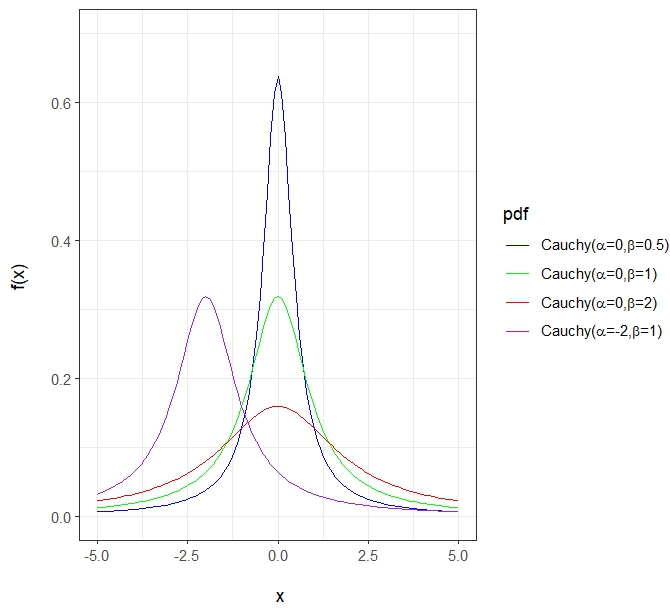
\includegraphics[scale=1]{Figuras/Cauchys.jpeg}
\caption{Distribuciones Cauchy.}
\end{figure}

\begin{theorem}
Si $X$ tiene distribución $Cauchy(\alpha ,\beta )$, entonces
\begin{equation*}
\begin{array}{l}
E(X)\text{ no existe} \\ 
V(X)\text{ no existe} \\ 
\text{La fgm no existe}
\end{array}
\end{equation*}
\end{theorem}

Veamos lo que pasa con la $E(X)$.
\begin{eqnarray*}
E(X) &=&\int_{-\infty }^{\infty }\frac{x}{\pi \beta \left[ 1+\left( \frac{%
x-\alpha }{\beta }\right) ^{2}\right] }dx \\
&=&\frac{1}{\pi \beta }\int_{-\infty }^{\infty }\frac{x}{\left[ 1+\frac{1}{%
\beta ^{2}}\left( x-\alpha \right) ^{2}\right] }dx \\
&=&\frac{1}{\pi \beta }\int_{-\infty }^{\infty }\frac{x}{\left[ \frac{\beta
^{2}+\left( x-\alpha \right) ^{2}}{\beta ^{2}}\right] }dx \\
&=&\frac{1}{\pi \beta }\int_{-\infty }^{\infty }\beta ^{2}\frac{x}{\beta
^{2}+(x-\alpha )^{2}}dx \\
&=&\frac{\beta }{\pi }\int_{-\infty }^{\infty }\frac{x}{\beta ^{2}+(x-\alpha
)^{2}}dx \\
&=&\frac{\beta }{\pi }\int_{-\infty }^{\infty }\frac{\alpha }{\beta
^{2}+(x-\alpha )^{2}}dx+\frac{\beta }{2\pi }\int_{-\infty }^{\infty }\frac{%
2(x-\alpha )}{\beta ^{2}+(x-\alpha )^{2}}dx
\end{eqnarray*}


En cuanto a la primera integral, se tiene que
\begin{eqnarray*}
\frac{\beta }{\pi }\int_{-\infty }^{\infty }\frac{\alpha }{\beta
^{2}+(x-\alpha )^{2}}dx &=&\frac{\beta \alpha }{\pi }\int_{-\infty }^{\infty
}\frac{dx}{\beta ^{2}+(x-\alpha )^{2}} \\
&=&\frac{\beta \alpha }{\pi }\int_{-\infty }^{\infty }\frac{dx/\beta ^{2}}{%
\left( \beta ^{2}+(x-\alpha )^{2}\right) /\beta ^{2}} \\
&=&\frac{\alpha }{\beta \pi }\int_{-\infty }^{\infty }\frac{dx}{1+(\frac{%
x-\alpha }{\beta })^{2}}\text{ //}\left( \arctan x\right) ^{\prime
}=1/(1+x^{2}) \\
&=&\frac{\alpha }{\beta \pi }\left. \arctan \left( \frac{x-\alpha }{\beta }%
\right) \right\vert _{-\infty }^{\infty } \\
&=&\frac{\alpha }{\beta \pi }\left( \frac{\pi }{2}-\left( -\frac{\pi }{2}%
\right) \right) = \\
&=&\frac{\alpha }{\beta \pi }\frac{2\pi }{2} \\
&=&\frac{\alpha }{\beta }
\end{eqnarray*}

Luego
\begin{eqnarray*}
E(X) &=&\frac{\beta }{\pi }\int_{-\infty }^{\infty }\frac{\alpha }{\beta
^{2}+(x-\alpha )^{2}}dx+\frac{\beta }{2\pi }\int_{-\infty }^{\infty }\frac{%
2(x-\alpha )}{\beta ^{2}+(x-\alpha )^{2}}dx \\
&=&\frac{\alpha }{\beta }+\frac{\beta }{2\pi }\int_{-\infty }^{\infty }\frac{%
2(x-\alpha )}{\beta ^{2}+(x-\alpha )^{2}}dx\text{ \ //}\frac{d}{dx}\ln
(f(x))=\frac{f{\acute{}}^{\prime }(x)}{f(x)} \\
&=&\frac{\alpha }{\beta }+\frac{\beta }{2\pi }\left. \ln \left[ \beta
^{2}+(x-\alpha )^{2}\right] \right\vert _{-\infty }^{\infty }
\end{eqnarray*}

Note que 
\begin{equation*}
\left. \ln \left[ \beta ^{2}+(x-\alpha )^{2}\right] \right\vert _{-\infty
}^{\infty }
\end{equation*}%
diverge cuando $x\rightarrow \infty $ ya que si $\ln (x)_{x\rightarrow
\infty }=\infty $ \ entonces\ $\ln (x^{2})_{x\rightarrow \infty }=\infty$.
Lo mismo pasa para cuando y $x\rightarrow -\infty $.
Por lo tanto $E(X)$ no existe.

Por otra parte $V(X)$ tampoco existe ya que $V(X)=E(X^{2})-\left[ E(X)\right]^{2}$ donde $E(X)$ no existe.

Finalmente la fgm de $X,$ que está dada por 
\begin{equation*}
m_{X}(t)=E(e^{tX})=\int_{-\infty }^{\infty }\frac{e^{tx}}{\pi \beta \left[
1+\left( \frac{x-\alpha }{\beta }\right) ^{2}\right] }dx
\end{equation*}%
no existe (\textbf{Tarea}).

Observación:
\begin{itemize}
\item Cuando la fgm no existe, entonces se puede utilizar la función
característica 
\begin{equation*}
\phi (t)=E(e^{itX})\text{, }-\infty <t<\infty
\end{equation*}%
donde $i=\sqrt{-1}$, la cual siempre existe y determina de manera única
la distribución de \ la v.a $X.$

\item Si la v.a $X$ tiene $n$-ésimo momento finito, entonces 
\begin{equation*}
\left. \frac{d^{n}}{dt^{n}}\phi (t)\right\vert _{t=0}=i^{n}E(X^{n})
\end{equation*}
\end{itemize}

\bigskip

%%%%%%%%%%%%%%%%%%%%%%%%%%%%%%%%%%%%
\subsection{*Lognormal}

\begin{definition}
Si $X$ es una v.a positiva tal que $Y=\ln X$, donde $Y$ tiene distribución normal, entonces $X$ tiene distribución lognormal si su pdf está dada por 
\begin{equation*}
f(x;\mu ,\sigma )=\frac{1}{x\sqrt{2\pi }\sigma }\exp \left[ -\frac{1}{%
2\sigma ^{2}}\left( \ln x-\mu \right) ^{2}\right] I_{(0,\infty )}(x)
\end{equation*}
donde $-\infty <\mu <\infty $, $\sigma >0.$ // $X\sim $lognormal$(\mu,\sigma )$
\end{definition}

\begin{theorem}
Si $X$ tiene distribución lognormal $(\mu ,\sigma )$,
entonces

\begin{equation*}
\begin{array}{l}
E(X)=e^{\mu +\sigma ^{2}/2} \\ 
V(X)=e^{2(\mu +\sigma ^{2})}-e^{2\mu +\sigma ^{2}} \\ 
\text{La fgm no existe}
\end{array}
\end{equation*}
\end{theorem}

Como $Y$ tiene distribución normal, note que
\begin{eqnarray*}
E(Y) &=&E(\ln X)=\mu \\
V(Y) &=&V(\ln X)=\sigma ^{2}
\end{eqnarray*}


Demostración:
\begin{eqnarray*}
E(X) &=&\int_{0}^{\infty }\frac{x}{x\sqrt{2\pi }\sigma }\exp \left[ -\frac{1%
}{2\sigma ^{2}}\left( \ln x-\mu \right) ^{2}\right] dx \\
&=&\int_{0}^{\infty }\frac{1}{\sqrt{2\pi }\sigma }\exp \left[ -\frac{1}{%
2\sigma ^{2}}\left( \ln x-\mu \right) ^{2}\right] dx
\end{eqnarray*}

Consideremos lo siguiente:
\begin{description}
\item[1)] Sea \ $y=\ln (x)-\mu $, donde $y\in (-\infty ,\infty ).$
\item[2)] Despejando para $\ln (x)$ en 1): $\ln (x)=y+\mu ,$
\item[3)] De 2) se tiene: $x=e^{y+\mu }$
\item[4)] Derivando 3) con respecto de $y:$ $dx=e^{y+\mu }dy$
\end{description}


\begin{eqnarray*}
E(X) &=&\int_{-\infty }^{\infty }\frac{1}{\sqrt{2\pi }\sigma }e^{\frac{-y^{2}
}{2\sigma ^{2}}}e^{y+\mu }dy \\
&=&\int_{-\infty }^{\infty }\frac{1}{\sqrt{2\pi }\sigma }e^{\frac{-y^{2}}{
2\sigma ^{2}}}e^{y}e^{\mu }dy \\
&=&e^{\mu }\int_{-\infty }^{\infty }\frac{1}{\sqrt{2\pi }\sigma }e^{\frac{-1
}{2\sigma ^{2}}(y^{2}-2y\sigma ^{2})}dy \\
&=&e^{\mu }\int_{-\infty }^{\infty }\frac{1}{\sqrt{2\pi }\sigma }e^{\frac{-1
}{2\sigma ^{2}}(y-\sigma ^{2})^{2}+\frac{\sigma ^{2}}{2}}dy \\
&=&e^{\mu +\frac{\sigma ^{2}}{2}}\int_{-\infty }^{\infty }\frac{1}{\sqrt{
2\pi }\sigma }e^{-\frac{1}{2\sigma ^{2}}(y-\sigma ^{2})^{2}}dy\text{ //}
Y\sim N(\sigma ^{2},\sigma ^{2}) \\
&=&e^{\mu +\frac{\sigma ^{2}}{2}}
\end{eqnarray*}
Luego
\begin{equation*}
E(X)=e^{\mu +\frac{\sigma ^{2}}{2}}
\end{equation*}

Por otra parte, consideremos nuevamente lo siguiente:
\begin{description}
\item[1)] Sea \ $y=\ln (x)-\mu $, donde $y\in (-\infty ,\infty ).$
\item[2)] Despejando para $\ln (x)$ en 1): $\ln (x)=y+\mu ,$
\item[3)] De 2) se tiene que: $x=e^{y+\mu }$
\item[4)] Derivando en 3) con respecto de $y:$ $dx=e^{y+\mu }dy$
\end{description}

\begin{eqnarray*}
E(X^{2}) &=&\int_{0}^{\infty }\frac{x^{2}}{x\sqrt{2\pi }\sigma }\exp \left[ -
\frac{1}{2\sigma ^{2}}\left( \ln x-\mu \right) ^{2}\right] dx \\
&=&\int_{0}^{\infty }\frac{x}{\sqrt{2\pi }\sigma }\exp \left[ -\frac{1}{
2\sigma ^{2}}\left( \ln x-\mu \right) ^{2}\right] dx \\
&=&\int_{-\infty }^{\infty }\frac{e^{y+\mu }}{\sqrt{2\pi }\sigma }e^{-\frac{
y^{2}}{2\sigma ^{2}}}e^{y+\mu }dy \\
&=&\int_{-\infty }^{\infty }\frac{1}{\sqrt{2\pi }\sigma }e^{y+\mu }e^{-\frac{
y^{2}}{2\sigma ^{2}}}e^{y+\mu }dy \\
&=&e^{2\mu }\int_{-\infty }^{\infty }\frac{1}{\sqrt{2\pi }\sigma }e^{-\frac{
y^{2}}{2\sigma ^{2}}}e^{2y}dy \\
&=&e^{2\mu }\int_{-\infty }^{\infty }\frac{1}{\sqrt{2\pi }\sigma }e^{-\frac{1
}{2\sigma ^{2}}(y^{2}-4y\sigma ^{2})}dy \\
&=&e^{2\mu }\int_{-\infty }^{\infty }\frac{1}{\sqrt{2\pi }\sigma }e^{-\frac{1
}{2\sigma ^{2}}(y-2\sigma ^{2})^{2}+2\sigma ^{2}}dy
\end{eqnarray*}%
Entonces%
\begin{equation*}
E(X^{2})=e^{2\mu +2\sigma ^{2}}\int_{-\infty }^{\infty }\frac{1}{\sqrt{2\pi }
\sigma }e^{-\frac{1}{2\sigma ^{2}}(y-2\sigma ^{2})^{2}}dy\text{ \ //}Y\sim
N(2\sigma ^{2},\sigma ^{2})
\end{equation*}

Luego 
\begin{equation*}
E(X^{2})=e^{2\mu +2\sigma ^{2}}
\end{equation*}

Entonces 
\begin{eqnarray*}
V(X) &=&E(X^{2})-\left[ E(X)\right] ^{2} \\
&=&e^{2\mu +2\sigma ^{2}}-\left( e^{\mu +\frac{\sigma ^{2}}{2}}\right) ^{2}
\\
&=&e^{2\left( \mu +\sigma ^{2}\right) }-e^{2\mu +\sigma ^{2}}
\end{eqnarray*}

De donde 
\begin{equation*}
V(X)=e^{2\left( \mu +\sigma ^{2}\right) }-e^{2\mu +\sigma ^{2}}
\end{equation*}


Note que que la varianza de $X$ también puede ser calculada con la
siguiente expresión:
\begin{eqnarray*}
V(X) &=&E\left[ \left( X-E(X)\right) ^{2}\right] \\
&=&\int \left( X-E(X)\right) ^{2}f(x)dx \\
&=&\int_{0}^{\infty }\frac{\left( x-e^{\mu +\frac{\sigma ^{2}}{2}}\right)
^{2}}{x\sqrt{2\pi }\sigma }\exp \left[ -\frac{1}{2\sigma ^{2}}\left( \ln
x-\mu \right) ^{2}\right] dx
\end{eqnarray*}


Finalmente para la fgm de $X$ que está dada por 
\begin{eqnarray*}
m_{X}(t) &=&E(e^{tX}) \\
&=&\int_{0}^{\infty }\frac{e^{tx}}{x\sqrt{2\pi }\sigma }\exp \left[ -\frac{1
}{2\sigma ^{2}}\left( \ln x-\mu \right) ^{2}\right] dx
\end{eqnarray*}%
No existe (\textbf{Tarea}).

%%%%%%%%%%%%%%%%%%%%%%%%%%%%%%%%%%%%%%%%%%%%%%%
\subsection{*Doble exponencial}

\begin{definition}
Una v.a $X$ tiene distribución doble exponencial o Laplace, si su función de densidad está dada por 
\begin{equation*}
f(x,\alpha ,\beta )=\frac{1}{2\beta }\exp \left( \frac{-\left\vert x-\alpha
\right\vert }{\beta }\right) I_{(-\infty ,\infty )}(x)
\end{equation*}%
donde $-\infty <\alpha <\infty $ y $\beta >0.$ //$X\sim Laplace(\alpha
,\beta )$
\end{definition}

\begin{theorem}
Si $X$ tiene distribución Laplace, entonces
\begin{eqnarray*}
E(X) &=&\alpha \\
V(X) &=&2\beta ^{2} \\
m_{X}(t) &=&\frac{e^{\alpha t}}{1-(\beta t)^{2}}\text{, \ \ \ }\left\vert
t\right\vert <1/\beta
\end{eqnarray*}
\end{theorem}

Demostración: 
\begin{equation*}
E(X)=\int_{-\infty }^{\infty }x\frac{1}{2\beta }\exp \left( \frac{%
-\left\vert x-\alpha \right\vert }{\beta }\right)dx
\end{equation*}

Note que 
\begin{equation*}
\left\vert x-\alpha \right\vert =\left\{ 
\begin{array}{c}
x-\alpha \text{, }x>\alpha \\ 
-(x-\alpha )\text{, }x<\alpha%
\end{array}%
\right.
\end{equation*}

Entonces

\begin{eqnarray*}
E(X) &=&\frac{1}{2\beta }\int_{-\infty }^{\alpha }x\exp \left( \frac{
x-\alpha }{\beta }\right) dx+\frac{1}{2\beta }\int_{\alpha }^{\infty }x\exp
\left( \frac{-(x-\alpha )}{\beta }\right) dx \\
&=&I+II
\end{eqnarray*}

\bigskip

Para $I$ se considera una integraci\'{o}n por partes: $\int uv^{\prime}=uv-\int u^{\prime }v$

\begin{equation*}
\begin{array}{ccc}
u=x &  & v^{\prime }=\exp \left( \frac{x-\alpha }{\beta }\right) \\ 
du=dx &  & v=\beta \exp \left( \frac{x-\alpha }{\beta }\right)%
\end{array}%
\end{equation*}

\bigskip

Entonces 
\begin{eqnarray*}
I &=&\frac{1}{2\beta }\int_{-\infty }^{\alpha }x\exp \left( \frac{x-\alpha }{
\beta }\right) dx \\
&=&\left. \frac{1}{2\beta }x\beta \exp \left( \frac{x-\alpha }{\beta }
\right) \right\vert _{-\infty }^{\alpha }-\frac{1}{2\beta }\int_{-\infty
}^{\alpha }\beta \exp \left( \frac{x-\alpha }{\beta }\right) dx \\
&=&\frac{\alpha }{2}-\frac{1}{2}\int_{-\infty }^{\alpha }\exp \left( \frac{
x-\alpha }{\beta }\right) dx\text{ \ //}u=\frac{x-\alpha }{\beta }\text{, \ }
du=\frac{1}{\beta }dx \\
&=&\frac{\alpha }{2}-\frac{\beta }{2}\int_{-\infty }^{\alpha }e^{u}du \\
&=&\frac{\alpha }{2}-\left. \frac{\beta }{2}\exp \left( \frac{x-\alpha }{
\beta }\right) \right\vert _{-\infty }^{\alpha } \\
&=&\frac{\alpha }{2}-\frac{\beta }{2}
\end{eqnarray*}


Para $II$ también se considera una integración por partes: $\int uv^{\prime }=uv-\int u^{\prime }v$

\begin{equation*}
\begin{array}{ccc}
u=x &  & v^{\prime }=\exp \left( \frac{-(x-\alpha )}{\beta }\right) \\ 
du=dx &  & v=-\beta \exp \left( \frac{-(x-\alpha )}{\beta }\right)
\end{array}%
\end{equation*}

Entonces
\begin{eqnarray*}
II &=&\frac{1}{2\beta }\int_{\alpha }^{\infty }x\exp \left( \frac{-(x-\alpha
)}{\beta }\right) dx \\
&=&\left. \frac{1}{2\beta }x(-\beta )\exp \left( \frac{-(x-\alpha )}{\beta }
\right) \right\vert _{\alpha }^{\infty }-\frac{1}{2\beta }\int_{\alpha
}^{\infty }-\beta \exp \left( \frac{-(x-\alpha )}{\beta }\right) dx \\
&=&\frac{1}{2\beta }\alpha \beta +\frac{1}{2}\int_{\alpha }^{\infty }\exp
\left( \frac{-(x-\alpha )}{\beta }\right) dx\text{ \ \ \ //}u=\frac{
-(x-\alpha )}{\beta }\text{, \ }du=\frac{-1}{\beta }dx \\
&=&\frac{\alpha }{2}-\frac{\beta }{2}\int_{\alpha }^{\infty }e^{u}du \\
&=&\frac{\alpha }{2}-\left. \frac{\beta }{2}\exp \left( \frac{-(x-\alpha )}{
\beta }\right) \right\vert _{\alpha }^{\infty } \\
&=&\frac{\alpha }{2}+\frac{\beta }{2}
\end{eqnarray*}

Luego 
\begin{eqnarray*}
E(X) &=&I+II \\
&=&\frac{\alpha }{2}-\frac{\beta }{2}+\frac{\alpha }{2}+\frac{\beta }{2} \\
&& \\
&=&\alpha
\end{eqnarray*}

Por otra parte
\begin{equation*}
E(X^{2})=\int_{-\infty }^{\infty }x^{2}\frac{1}{2\beta }\exp \left( \frac{-\left\vert x-\alpha \right\vert }{\beta }\right) dx
\end{equation*}

Note que 
\begin{equation*}
\left\vert x-\alpha \right\vert =\left\{ 
\begin{array}{c}
x-\alpha \text{, }x>\alpha \\ 
-(x-\alpha )\text{, }x<\alpha
\end{array}
\right.
\end{equation*}

Entonces
\begin{eqnarray*}
E(X^{2}) &=&\frac{1}{2\beta }\int_{-\infty }^{\alpha }x^{2}\exp \left( \frac{
x-\alpha }{\beta }\right) dx+\frac{1}{2\beta }\int_{\alpha }^{\infty
}x^{2}\exp \left( \frac{-(x-\alpha )}{\beta }\right) dx \\
&=&I+II
\end{eqnarray*}

Para $I$ se considera una integración por partes: $\int uv^{\prime}=uv-\int u^{\prime }v$

$u=x^{2},$ \ $\ \ \ \ v^{\prime }=\exp \left( \frac{x-\alpha }{\beta}\right) $

$du=2xdx$, \ \ $v=\beta \exp \left( \frac{x-\alpha }{\beta }\right) $

Entonces 
\begin{eqnarray*}
I &=&\frac{1}{2\beta }\int_{-\infty }^{\alpha }x^{2}\exp \left( \frac{
x-\alpha }{\beta }\right) dx \\
&=&\left. \frac{1}{2\beta }x^{2}\beta \exp \left( \frac{x-\alpha }{\beta }
\right) \right\vert _{-\infty }^{\alpha }-\frac{1}{2\beta }\int_{-\infty
}^{\alpha }2x\beta \exp \left( \frac{x-\alpha }{\beta }\right) dx \\
&=&\frac{\alpha ^{2}}{2}-\int_{-\infty }^{\alpha }x\exp \left( \frac{
x-\alpha }{\beta }\right) dx\text{ \ }
\end{eqnarray*}

Consideremos nuevamente una integración por partes,
$u=x,$ \ $\ \ \ \ v^{\prime }=\exp \left( \frac{x-\alpha }{\beta }\right) $
$du=dx$, \ \ $v=\beta \exp \left( \frac{x-\alpha }{\beta }\right) $

Entonces
\begin{eqnarray*}
I &=&\frac{\alpha ^{2}}{2}-\int_{-\infty }^{\alpha }x\exp \left( \frac{
x-\alpha }{\beta }\right) dx\text{ \ } \\
&=&\frac{\alpha ^{2}}{2}-\left[ \left. x\beta \exp \left( \frac{x-\alpha }{
\beta }\right) \right\vert _{-\infty }^{\alpha }-\int_{-\infty }^{\alpha
}\beta \exp \left( \frac{x-\alpha }{\beta }\right) dx\right] \\
&=&\frac{\alpha ^{2}}{2}-\alpha \beta +\beta ^{2}\int_{-\infty }^{\alpha
}\exp \left( \frac{x-\alpha }{\beta }\right) dx\text{ //}u=\frac{x-\alpha }{
\beta }\text{, \ }du=\frac{1}{\beta }dx \\
&=&\frac{\alpha ^{2}}{2}-\alpha \beta +\beta ^{2}\int_{-\infty }^{\alpha
}e^{u}du \\
&=&\frac{\alpha ^{2}}{2}-\alpha \beta +\beta ^{2}\left[ \left. \exp \left( 
\frac{x-\alpha }{\beta }\right) \right\vert _{-\infty }^{\alpha }\right] \\
&=&\frac{\alpha ^{2}}{2}-\alpha \beta +\beta ^{2} \\
&=&\frac{\alpha ^{2}}{2}-\alpha \beta +\beta ^{2}
\end{eqnarray*}

\bigskip

Para la parte $II$, consideramos también una integración por partes: 
$\int uv^{\prime }=uv-\int u^{\prime }v$

$u=x^{2},$ \ $\ \ \ \ v^{\prime }=\exp \left( \frac{-(x-\alpha )}{\beta }\right)$

$du=2xdx$, \ \ $v=-\beta \exp \left( \frac{-(x-\alpha )}{\beta }\right) $

Entonces
\begin{eqnarray*}
II &=&\frac{1}{2\beta }\int_{\alpha }^{\infty }x^{2}\exp \left( \frac{
-(x-\alpha )}{\beta }\right) dx \\
&=&\left. \frac{1}{2\beta }x^{2}(-\beta )\exp \left( \frac{-(x-\alpha )}{
\beta }\right) \right\vert _{\alpha }^{\infty }-\frac{1}{2\beta }
\int_{\alpha }^{\infty }-2x\beta \exp \left( \frac{-(x-\alpha )}{\beta }
\right) dx \\
&=&\frac{1}{2\beta }\alpha ^{2}\beta +\int_{\alpha }^{\infty }x\exp \left( 
\frac{-(x-\alpha )}{\beta }\right) dx\text{ \ \ } \\
&=&\frac{\alpha ^{2}}{2}+\int_{\alpha }^{\infty }x\exp \left( \frac{
-(x-\alpha )}{\beta }\right) dx\text{ \ \ }
\end{eqnarray*}

Volvemos a realizar integración por partes: $\int uv^{\prime }=uv-\int u^{\prime }v$

$u=x,$ \ $\ \ \ \ v^{\prime }=\exp \left( \frac{-(x-\alpha )}{\beta }\right) $
$du=dx$, \ \ $v=-\beta \exp \left( \frac{-(x-\alpha )}{\beta }\right) $

\begin{eqnarray*}
II &=&\frac{\alpha ^{2}}{2}+\int_{\alpha }^{\infty }x\exp \left( \frac{
-(x-\alpha )}{\beta }\right) dx\text{ \ \ } \\
&=&\frac{\alpha ^{2}}{2}+\left. x(-\beta )\exp \left( \frac{-(x-\alpha )}{
\beta }\right) \right\vert _{\alpha }^{\infty }-\int_{\alpha }^{\infty
}-\beta \exp \left( \frac{-(x-\alpha )}{\beta }\right) dx \\
&=&\frac{\alpha ^{2}}{2}+\alpha \beta +\beta \int_{\alpha }^{\infty }\exp
\left( \frac{-(x-\alpha )}{\beta }\right) dx\text{ \ \ \ //}u=\frac{
-(x-\alpha )}{\beta }\text{, \ }du=\frac{-1}{\beta }dx \\
&=&\frac{\alpha ^{2}}{2}+\alpha \beta -\beta ^{2}\int_{\alpha }^{\infty
}e^{u}du \\
&=&\frac{\alpha ^{2}}{2}+\alpha \beta -\beta ^{2}\left. \exp \left( \frac{
-(x-\alpha )}{\beta }\right) \right\vert _{\alpha }^{\infty } \\
&=&\frac{\alpha ^{2}}{2}+\alpha \beta +\beta ^{2}
\end{eqnarray*}

Luego
\begin{equation*}
II=\frac{\alpha ^{2}}{2}+\alpha \beta +\beta ^{2}
\end{equation*}%
Entonces 
\begin{eqnarray*}
E(X^{2}) &=&I+II \\
&=&\frac{\alpha ^{2}}{2}-\alpha \beta +\beta ^{2}+\frac{\alpha ^{2}}{2}%
+\alpha \beta +\beta ^{2} \\
&=&\alpha ^{2}+2\beta ^{2}
\end{eqnarray*}

Finalmente
\begin{eqnarray*}
V(X) &=&E(X^{2})-[E(X)]^{2} \\
&=&\alpha ^{2}+2\beta ^{2}-\alpha ^{2} \\
&=&2\beta ^{2}
\end{eqnarray*}

Por lo tanto 
\begin{equation*}
V(X)=2\beta ^{2}
\end{equation*}

Por otra parte, la fgm de $X$ se encuentra resolviendo la siguiente integral
\begin{eqnarray*}
m_{X}(t) &=&E(e^{tX}) \\
&=&\int_{-\infty }^{\infty }e^{xt}\frac{1}{2\beta }\exp \left( \frac{
-\left\vert x-\alpha \right\vert }{\beta }\right) dx \\
&=&\int_{-\infty }^{\alpha }e^{xt}\frac{1}{2\beta }\exp \left( \frac{
x-\alpha }{\beta }\right) dx+\int_{\alpha }^{\infty }e^{xt}\frac{1}{2\beta }
\exp \left( \frac{-(x-\alpha )}{\beta }\right) dx
\end{eqnarray*}

\textbf{Tarea: }Determinar que 
\begin{equation*}
m_{X}(t)=\frac{e^{\alpha t}}{1-(\beta t)^{2}}\text{, \ \ \ }\left\vert
t\right\vert <1/\beta
\end{equation*}

%%%%%%%%%%%%%%%%%%%%%%%%%%%%%%%%%%%%%
\subsection{Weibull}

\begin{definition}
Una v.a $X$ tiene distribución Weibull si su pdf está dada por
\begin{equation*}
f(x,a,b)=abx^{b-1}e^{-ax^{b}}I_{(0,\infty )}(x)
\end{equation*}%
con $a>0,$ $b>0$. // $X\sim Weibull(a,b)$
\end{definition}

Observaciones:
\begin{itemize}
\item Para $b=1$
\begin{equation*}
f(x,a,b)=ae^{-ax}I_{(0,\infty )}(x)
\end{equation*}
se tiene la distribución exponencial.

\item La Weibull, pertenece a la familia de valores extremos generalizada compuesta por la distribución Gumbel, Fréchet y Weibull (Coles, $2001$).

\item La Gompertz pertenece al dominio de atracción de la Wiebull.
\end{itemize}

\begin{figure}[h!]
\centering
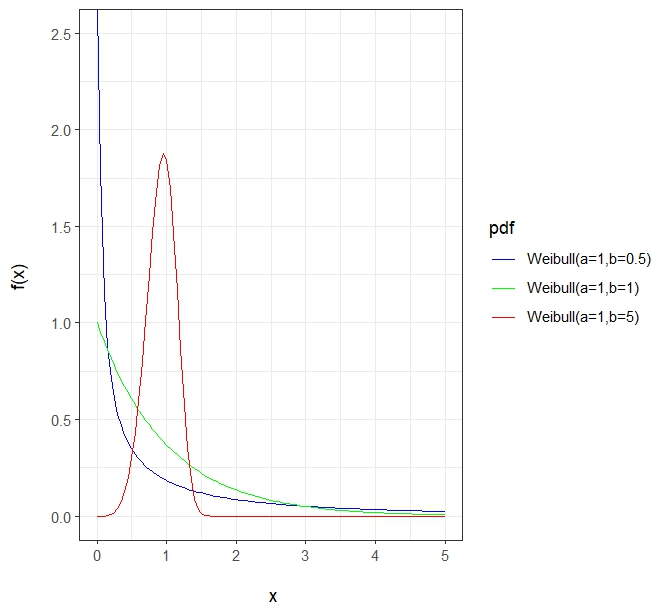
\includegraphics[scale=1]{Figuras/Weibulls.jpeg}
\caption{Distribuciones Weibulls.}
\end{figure}

\begin{theorem}
Si $X$ tiene distribución $Weibull(a,b)$, entonces
\begin{eqnarray*}
E(X) &=&\left( \frac{1}{a}\right) ^{1/b}\Gamma \left( 1+\frac{1}{b}\right) \\
V(X) &=&\left( \frac{1}{a}\right) ^{2/b}\left[ \Gamma \left( 1+\frac{2}{b}
\right) -\Gamma ^{2}\left( 1+\frac{1}{b}\right) \right]
\end{eqnarray*}
\end{theorem}

Observación: La fgm solo existe para $b\geq 1$.
Calculo de la esperanza de $X$: 
\begin{equation*}
E(X)=\int_{0}^{\infty }xabx^{b-1}e^{-ax^{b}}dx
\end{equation*}

Sea
\begin{enumerate}
\item[1)] $u=ax^{b}$, \ 
\item[2)] Despejando para $x$ de 1):\ $x=\left( \frac{u}{a}\right) ^{1/b}$
\item[3)] Derivando 1) con respecto de $x:$ $\ du=abx^{b-1}dx$
\end{enumerate}

Entonces
\begin{eqnarray*}
E(X) &=&\int_{0}^{\infty }\left( \frac{u}{a}\right) ^{1/b}e^{-u}du \\
&=&\left( \frac{1}{a}\right) ^{1/b}\int_{0}^{\infty }u^{1/b}e^{-u}du \\
&=&\left( \frac{1}{a}\right) ^{1/b}\int_{0}^{\infty }u^{(1/b+1)-1}e^{-u}du
\text{ \ \ //}\Gamma (t)=\int_{0}^{\infty }x^{t-1}e^{-x}dx \\
&=&\left( \frac{1}{a}\right) ^{1/b}\Gamma \left( \frac{1}{b}+1\right)
\end{eqnarray*}

Luego 
\begin{equation*}
E(X)=\left( \frac{1}{a}\right) ^{1/b}\Gamma \left( \frac{1}{b}+1\right)
\end{equation*}

Por otra parte,
\begin{equation*}
E(X^{2})=\int_{0}^{\infty }x^{2}abx^{b-1}e^{-ax^{b}}dx
\end{equation*}

Considerando el siguiente cambio de variable:
\begin{enumerate}
\item[1)] $u=ax^{b}$

\item[2)] Despejando para $x$ de 1): $x=\left( \frac{u}{a}\right) ^{1/b}$

\item[3)] Derivando 1) con respecto de $x:$ $du=abx^{b-1}dx$
\end{enumerate}


Entonces 
\begin{eqnarray*}
E(X^{2}) &=&\int_{0}^{\infty }x^{2}abx^{b-1}e^{-ax^{b}}dx \\
&=&\int_{0}^{\infty }\left( \frac{u}{a}\right) ^{2/b}e^{-u}du \\
&=&\left( \frac{1}{a}\right) ^{2/b}\int_{0}^{\infty }u^{(2/b+1)-1}e^{-u}du
\text{ \ \ \ //}\Gamma (t)=\int_{0}^{\infty }x^{t-1}e^{-x}dx \\
E(X^{2}) &=&\left( \frac{1}{a}\right) ^{2/b}\Gamma \left( \frac{2}{b}
+1\right)
\end{eqnarray*}

Luego 
\begin{eqnarray*}
V(X) &=&\left( \frac{1}{a}\right) ^{2/b}\Gamma \left( \frac{2}{b}+1\right)
-\left( \frac{1}{a}\right) ^{2/b}\Gamma ^{2}\left( \frac{1}{b}+1\right) \\
&=&\left( \frac{1}{a}\right) ^{2/b}\left[ \Gamma \left( \frac{2}{b}+1\right)
-\Gamma ^{2}\left( \frac{1}{b}+1\right) \right]
\end{eqnarray*}

Para conocer más sobre la distribución Weibull ver Rinne ($2008$) y el Capítulo 21 del Johnson \& Balakrishnan ($1994$).


%%%%%%%%%%%%%%%%%%%%%%%%%%%%%%%%%%%%%%%%%%%%
\subsection{*Logística}


\begin{definition}
 Una v.a $X$ tiene distribución logística($\alpha ,\beta $) si su pdf está dada por 
\begin{equation*}
f(x;\alpha ,\beta )=\frac{1}{\beta }\frac{\exp \left( \frac{-(x-\alpha )}{
\beta }\right) }{\left[ 1+\exp \left( \frac{-(x-\alpha )}{\beta }\right) 
\right] ^{2}}I_{(-\infty ,\infty )}(x)\text{ }
\end{equation*}%
$-\infty <\alpha <\infty $, $\beta >0$. // $X\sim $logística($\alpha
,\beta $)
\end{definition}


\begin{theorem}
Si $X$ tiene distribución logística($\alpha,\beta $), entonces
\begin{eqnarray*}
E(X) &=&\alpha \\
V(X) &=&\frac{\pi ^{2}\beta ^{2}}{3} \\
m_{X}(t) &=&e^{\alpha t}\pi \beta t\csc \left( \pi \beta t\right) .
\end{eqnarray*}    
\end{theorem}


Observación: Si la v.a $X$ tiene distribución logística,
entonces es simétrica respecto a $\alpha $.

\textbf{Demostración}:
Note que 
\begin{equation*}
E(X)=\int_{-\infty }^{\infty }\frac{x}{\beta }\frac{e^{-\left( \frac{
x-\alpha }{\beta }\right) }}{\left[ 1+\exp \left( -\frac{(x-\alpha )}{\beta }
\right) \right] ^{2}}dx
\end{equation*}

Considerando:
\begin{enumerate}
\item[1)] $y=\frac{x-\alpha }{\beta }$
\item[2)] Despejando para $x$ de 1): $x=\beta y+\alpha .$
\item[3)] Derivando 1) con respecto a $x$: $dy=\frac{dx}{\beta }$.
\end{enumerate}

\begin{eqnarray*}
E(X) &=&\int_{-\infty }^{\infty }(\alpha +\beta y)\frac{e^{-y}}{\left[
1+e^{-y}\right] ^{2}}dy \\
&=&\alpha \int_{-\infty }^{\infty }\frac{e^{-y}}{\left[ 1+e^{-y}\right] ^{2}}
dy+\beta \int_{-\infty }^{\infty }y\frac{e^{-y}}{\left[ 1+e^{-y}\right] ^{2}}
dy \\
&=&\alpha \int_{-\infty }^{\infty }\frac{1}{\beta }\frac{\exp \left( -\frac{
x-\alpha }{\beta }\right) }{\left[ 1+\exp \left( \frac{-(x-\alpha )}{\beta }
\right) \right] ^{2}}dx+\beta \int_{-\infty }^{\infty }y\frac{e^{-y}}{\left[
1+e^{-y}\right] ^{2}}dy\text{ //}X\sim \text{logística(}\alpha ,\beta 
\text{)} \\
&=&\alpha \cdot 1+\beta \int_{-\infty }^{\infty }y\frac{e^{-y}}{\left[
1+e^{-y}\right] ^{2}}dy
\end{eqnarray*}


Para la segunda integral se considera:

\begin{description}
\item[1)] $z=\frac{1}{1+e^{-y}}$,

\item[2)] Derivando $1$) con respecto de $y:$ $dz=\frac{e^{-y}}{\left(
1+e^{-y}\right) ^{2}}dy$ \ 

\item[3)] Despejando\ para $y$ de 1) y tomando el logaritmo se tiene: $y=\ln
\left( \frac{z}{1-z}\right) $
\end{description}

Entonces 
\begin{eqnarray*}
\beta \int_{-\infty }^{\infty }y\frac{e^{-y}}{\left[ 1+e^{-y}\right] ^{2}}dy
&=&\beta \int_{0}^{1}\ln \left( \frac{z}{1-z}\right) dz \\
&=&\beta \int_{0}^{1}\ln \left( z\right) dz-\beta \int_{0}^{1}\ln \left(
1-z\right) dz\text{ //Propiedad} \\
&=&\beta \int_{0}^{1}\ln \left( z\right) dz-\beta \int_{0}^{1}\ln \left(
t\right) dt\text{ \ //}t=1-z \\
&=&\beta \ast 0-\beta \ast 0 \\
&=&0
\end{eqnarray*}

Luego
\begin{eqnarray*}
E(X) &=&\alpha +\beta \int_{-\infty }^{\infty }y\frac{e^{-y}}{\left[ 1+e^{-y}
\right] ^{2}}dy \\
&=&\alpha +0 \\
&=&\alpha
\end{eqnarray*}%
Por lo tanto 
\begin{equation*}
E(X)=\alpha .
\end{equation*}


Por otra parte,
\begin{equation*}
E(X^{2})=\int_{-\infty }^{\infty }\frac{x^{2}}{\beta }\frac{e^{-\left( \frac{
x-\alpha }{\beta }\right) }}{\left[ 1+\exp \left( -\frac{(x-\alpha )}{\beta }
\right) \right] ^{2}}dx
\end{equation*}

\textbf{Tarea}. Probar que 
\begin{equation*}
V(X)=\frac{\pi ^{2}\beta ^{2}}{3}
\end{equation*}

%%%%%%%%%%%%%%%%%%%%%%%%%%%%%%%%%%%%
\subsection{*Pareto}

\begin{definition}
Una v.a $X$ tiene distribución Pareto si su pdf está dada por
\begin{eqnarray*}
f(x,x_{0},\theta ) &=&\frac{\theta }{x_{0}}\left( \frac{x_{0}}{x}\right)
^{\theta +1}I_{(x_{0},\infty )}(x) \\
&=&\frac{\theta x_{0}^{\theta }}{x^{\theta +1}}I_{(x_{0},\infty )}(x)
\end{eqnarray*}%
donde $\theta >0$ y $x_{0}>0$. //$X\sim Pareto(x_{0},\theta )$
\end{definition}

\begin{theorem}
Si $X$ tiene distribución $Pareto(x_{0},\theta )$, entonces
\begin{equation*}
\begin{array}{l}
E(X)=\frac{\theta x_{0}}{\theta -1},\text{ \ }\theta >1 \\ 
\\ 
V(X)=\frac{\theta x_{0}^{2}}{\theta -2}-\left( \frac{\theta x_{0}}{\theta -1}
\right) ^{2}\text{, }\theta >2 \\ 
\\ 
\text{La fgm no existe.}
\end{array}
\end{equation*}
\end{theorem}

Demostración
\begin{eqnarray*}
E(X^{k}) &=&\int_{x_{0}}^{\infty }x^{k}\frac{\theta }{x_{0}}\frac{
x_{0}^{\theta +1}}{x^{\theta +1}}dx \\
&=&\theta x_{0}^{\theta +1}\int_{x_{0}}^{\infty }x^{k}\frac{1}{x_{0}}\frac{1
}{x^{\theta +1}}dx \\
&=&\theta x_{0}^{\theta +1}\int_{x_{0}}^{\infty }\frac{1}{x_{0}}\frac{1}{
x^{\theta -k+1}}dx \\
&=&\frac{\theta x_{0}^{\theta +1}}{x_{0}^{\theta -k+1}(\theta -k)}
\int_{x_{0}}^{\infty }\frac{(\theta -k)}{x_{0}}\frac{x_{0}^{\theta -k+1}}{
x^{\theta -k+1}}dx\text{ //}pdf\text{ pareto} \\
&=&\frac{\theta x_{0}^{\theta +1}}{x_{0}^{\theta -k+1}(\theta -k)}
\int_{x_{0}}^{\infty }\frac{(\theta -k)}{x_{0}}\left( \frac{x_{0}}{x}\right)
^{(\theta -k)+1}dx\text{ //}pdf\text{ pareto} \\
&=&\frac{\theta x_{0}^{\theta +1}}{x_{0}^{\theta -k+1}(\theta -k)} \\
&=&\frac{\theta x_{0}^{k}}{\theta -k}
\end{eqnarray*}%
i.e,
\begin{equation*}
E(X^{k})=\frac{\theta x_{0}^{k}}{\theta -k}
\end{equation*}

Para $k=1$
\begin{equation*}
E(X)=\frac{\theta x_{0}}{\theta -1},\text{ }\theta >1\text{\ }
\end{equation*}

Para $k=2$,
\begin{equation*}
E(X^{2})=\frac{\theta x_{0}^{2}}{\theta -2}\text{, }\theta >2
\end{equation*}%
Entonces
\begin{eqnarray*}
V(X) &=&E(X^{2})-(E(X))^{2} \\
&=&\frac{\theta x_{0}^{2}}{\theta -2}-\left( \frac{\theta x_{0}}{\theta -1}
\right) ^{2}\text{, \ }\theta >2
\end{eqnarray*}

%%%%%%%%%%%%%%%%%%%%%%%%%%%%%%%%%%%%%%%%%%
\subsection{t de Student}

\begin{definition}
Una v.a $X$ tiene distribución t de Studen con $v$ grados de libertad, si su pdf está dada por
\begin{equation*}
f(x;v)=\frac{\Gamma \left( \frac{v+1}{2}\right) }{\Gamma \left( \frac{v}{2}
\right) \sqrt{v\pi }}\left( 1+\frac{x^{2}}{v}\right) ^{-\left( \frac{v+1}{2}
\right) }I_{(-\infty ,\infty )}(x)
\end{equation*}%
con $v>0$ // $X\sim t(v)$.
\end{definition}

\begin{figure}[h!]
\centering
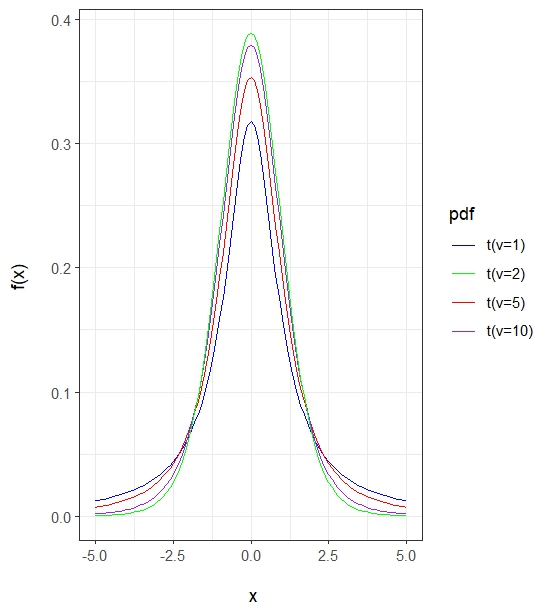
\includegraphics[scale=1]{Figuras/t_students.jpeg}
\caption{Distribuciones t de Student.}
\end{figure}

\begin{theorem}
Si $X$ tiene distribución $t(v)$, entonces
\begin{equation*}
\begin{array}{l}
E(X)=0\text{, \ }v>1 \\ 
\\ 
V(X)=\frac{v}{v-2},\text{ }v>2 \\ 
\\ 
\text{La fgm no existe.}
\end{array}
\end{equation*}
\end{theorem}


Dado que la $t$ de Student es simétrica respecto al origen, entonces
\begin{equation*}
E(X)=0
\end{equation*}


Por otra parte,
\begin{eqnarray*}
E(X^{2}) &=&\int_{-\infty }^{\infty }x^{2}\frac{\Gamma \left( \frac{v+1}{2}
\right) }{\Gamma \left( \frac{v}{2}\right) \sqrt{v\pi }}\left( 1+\frac{x^{2}
}{v}\right) ^{-\left( \frac{v+1}{2}\right) }dx \\
&=&2\int_{0}^{\infty }x^{2}\frac{\Gamma \left( \frac{v+1}{2}\right) }{\Gamma
\left( \frac{v}{2}\right) \sqrt{v\pi }}\left( 1+\frac{x^{2}}{v}\right)
^{-\left( \frac{v+1}{2}\right) }dx\text{// simetr\'{\i}a de la }t \\
&=&2\frac{\Gamma \left( \frac{v+1}{2}\right) }{\Gamma \left( \frac{v}{2}
\right) \sqrt{v\pi }}\int_{0}^{\infty }x^{2}\left( 1+\frac{x^{2}}{v}\right)
^{-\left( \frac{v+1}{2}\right) }dx\text{ }
\end{eqnarray*}


Cambio de variable:
\begin{enumerate}
\item[1)] Sea $u=\frac{x^{2}}{v}$

\item[2)] Despejado para $x$ de 1): $x=\sqrt{uv}$

\item[3)] De 1) derivar $u$ con respecto de $x$: $du=\frac{2x}{v}dx$,

\item[4)] Despejado para $dx$ en 3): $dx=\frac{du}{2x}v$

\item[5)] Sustituyendo 2) en 4): $dx=\frac{vdu}{2\sqrt{uv}}=\frac{\sqrt{v}du
}{2\sqrt{u}}$
\end{enumerate}

Entonces
\begin{eqnarray*}
E(X^{2}) &=&\frac{2\Gamma \left( \frac{v+1}{2}\right) }{\Gamma \left( \frac{v
}{2}\right) \sqrt{v\pi }}\int_{0}^{\infty }uv\left( 1+u\right) ^{-\left( 
\frac{v+1}{2}\right) }\frac{\sqrt{v}du}{2\sqrt{u}} \\
&=&\frac{2\Gamma \left( \frac{v+1}{2}\right) }{\Gamma \left( \frac{v}{2}
\right) \sqrt{v\pi }}\frac{v^{3/2}}{2}\int_{0}^{\infty }u^{1/2}\left(
1+u\right) ^{-\left( \frac{v+1}{2}\right) }du \\
&=&\frac{2\Gamma \left( \frac{v+1}{2}\right) }{\Gamma \left( \frac{v}{2}
\right) \sqrt{v}\sqrt{\pi }}\frac{v^{3/2}}{2}\int_{0}^{\infty }\frac{u^{1/2}
}{\left( 1+u\right) ^{\left( \frac{v+1}{2}\right) }}du \\
&=&\frac{\Gamma \left( \frac{v+1}{2}\right) }{\Gamma \left( \frac{v}{2}
\right) }\frac{v}{\sqrt{\pi }}\int_{0}^{\infty }\frac{u^{3/2-1}}{\left(
1+u\right) ^{3/2+\left( \frac{v}{2}-1\right) }}du\text{ \ //}B(\alpha,\beta
)=\int_{0}^{\infty }\frac{x^{\alpha -1}}{(1+x)^{\alpha +\beta }}dx \\
&=&\frac{\Gamma \left( \frac{v+1}{2}\right) }{\Gamma \left( \frac{v}{2}
\right) }\frac{v}{\sqrt{\pi }}B\left( 3/2,v/2-1\right)
\end{eqnarray*}

i.e,
\begin{eqnarray*}
E(X^{2}) &=&\frac{\Gamma \left( \frac{v+1}{2}\right) }{\Gamma \left( \frac{v
}{2}\right) }\frac{v}{\sqrt{\pi }}\frac{\Gamma (3/2)\Gamma (v/2-1)}{\Gamma
\left( \frac{v+1}{2}\right) } \\
&=&v\frac{\Gamma (3/2)\Gamma (v/2-1)}{\Gamma \left( v/2\right) \sqrt{\pi }}
\text{ \ \ \ //}\Gamma (3/2)=\frac{\sqrt{\pi }}{2} \\
&=&v\frac{\frac{\sqrt{\pi }}{2}\Gamma (v/2-1)}{\Gamma \left( v/2\right) 
\sqrt{\pi }} \\
&=&\frac{v}{2}\frac{\Gamma (v/2-1)}{\Gamma \left( v/2\right) } \\
&=&\frac{v}{2\left( \frac{v}{2}-1\right) } \\
&=&\frac{v}{v-2}\text{, \ \ \ }v>2.
\end{eqnarray*}

Luego
\begin{equation*}
E(X^{2})=\frac{v}{v-2}\text{, \ \ \ }v>2.
\end{equation*}
Entonces%
\begin{eqnarray*}
V(X) &=&E(X^{2})-\left[ E(X)\right] ^{2} \\
&=&\frac{v}{v-2}-0 \\
&=&\frac{v}{v-2}
\end{eqnarray*}

Por lo tanto 
\begin{equation*}
V(X)=\frac{v}{v-2}
\end{equation*}
para $v>2$.

%%%%%%%%%%%%%%%%%%%%%%%%%%%%%%%%%%%%%%%%%%
\subsection{*F}